\section{Anàlisi i modelatge Geoespacial}


Per poder fer la nostra anàlisi i modelatge Geospacial, s'han necessitat les coordenades de les nostres dades. Al principi del projecte ja es va fer un preprocess de les nostres dades i es van trobar el país i la ciutat d'origen de tots els artistes de la base de dades. Per aquest apartat s'ha fet servir una API, per aconseguir la latitud i la longitud d'aquestes ciutats.

Cal destacar que prèviament a importar les coordenades mitjançant l'API, s'han modificat algunes files per tal que aquesta API funcioni correctament per totes les files.

Ens vam adonar que el país de Puerto Rico no era detectat correctament i que hi havia ciutats que eren NA. A més, hi havia artistes que tenien com a ciutat una que no era correcte, per tant, es va canviar tota aquesta informació.

Un cop ja tenim tots els països i ciutats correctament de cada artista, s'ha utilitzat l'API de la web Geocoding, que dona les coordenades de cada ciutat quan es proporciona el nom de la ciutat i del país.

Finalment, obtenim un nou conjunt de dades amb les variables de latitud i longitud dels artistes.

% MODELATGE
Amb aquestes dades aconseguides, s'ha procedit a fer l'anàlisi i modelatge geoespacial. Es presentaran els mètodes d'anàlisi geoespacial aplicats al nostre dataset. Els mètodes geoespacials es poden classificar en dues categories principals: l'anàlisi de dades tipus I i l'anàlisi de dades tipus II. A continuació, es descriuen aquestes dues categories i s'analitzen els resultats corresponents amb les nostres dades.

\subsection{Anàlisi Geoespacial Tipus II: Procesos Puntuals Específics}

Aquest tipus d'anàlisi se centra en l'estudi de la distribució espacial de l'ocurrència d'esdeveniments. D'aquí podrem extreure conclusions sobre si l'aparició dels esdeveniments (en el nostre cas seran característiques de les nostres cançons o artistes) és uniforme en l'espai o si hi ha àrees on els esdeveniments tendeixen a ocórrer amb més o menys freqüència. \\

Com s'ha mencionat anteriorment, nosaltres comptem amb les coordenades de cada artista, el lloc d'on són cadascun. Primer de tot, visualitzarem aquests punts. En la primera Figura \ref{fig:geo_mapa_punts} veiem en verd tots els artistes de la nostra database. En la segona, podem veure un mapa d'intensitat per observar a quines zones del món es concentren més artistes \ref{fig:geo_mapa_den}. \\

\begin{figure}[H]
    \centering
    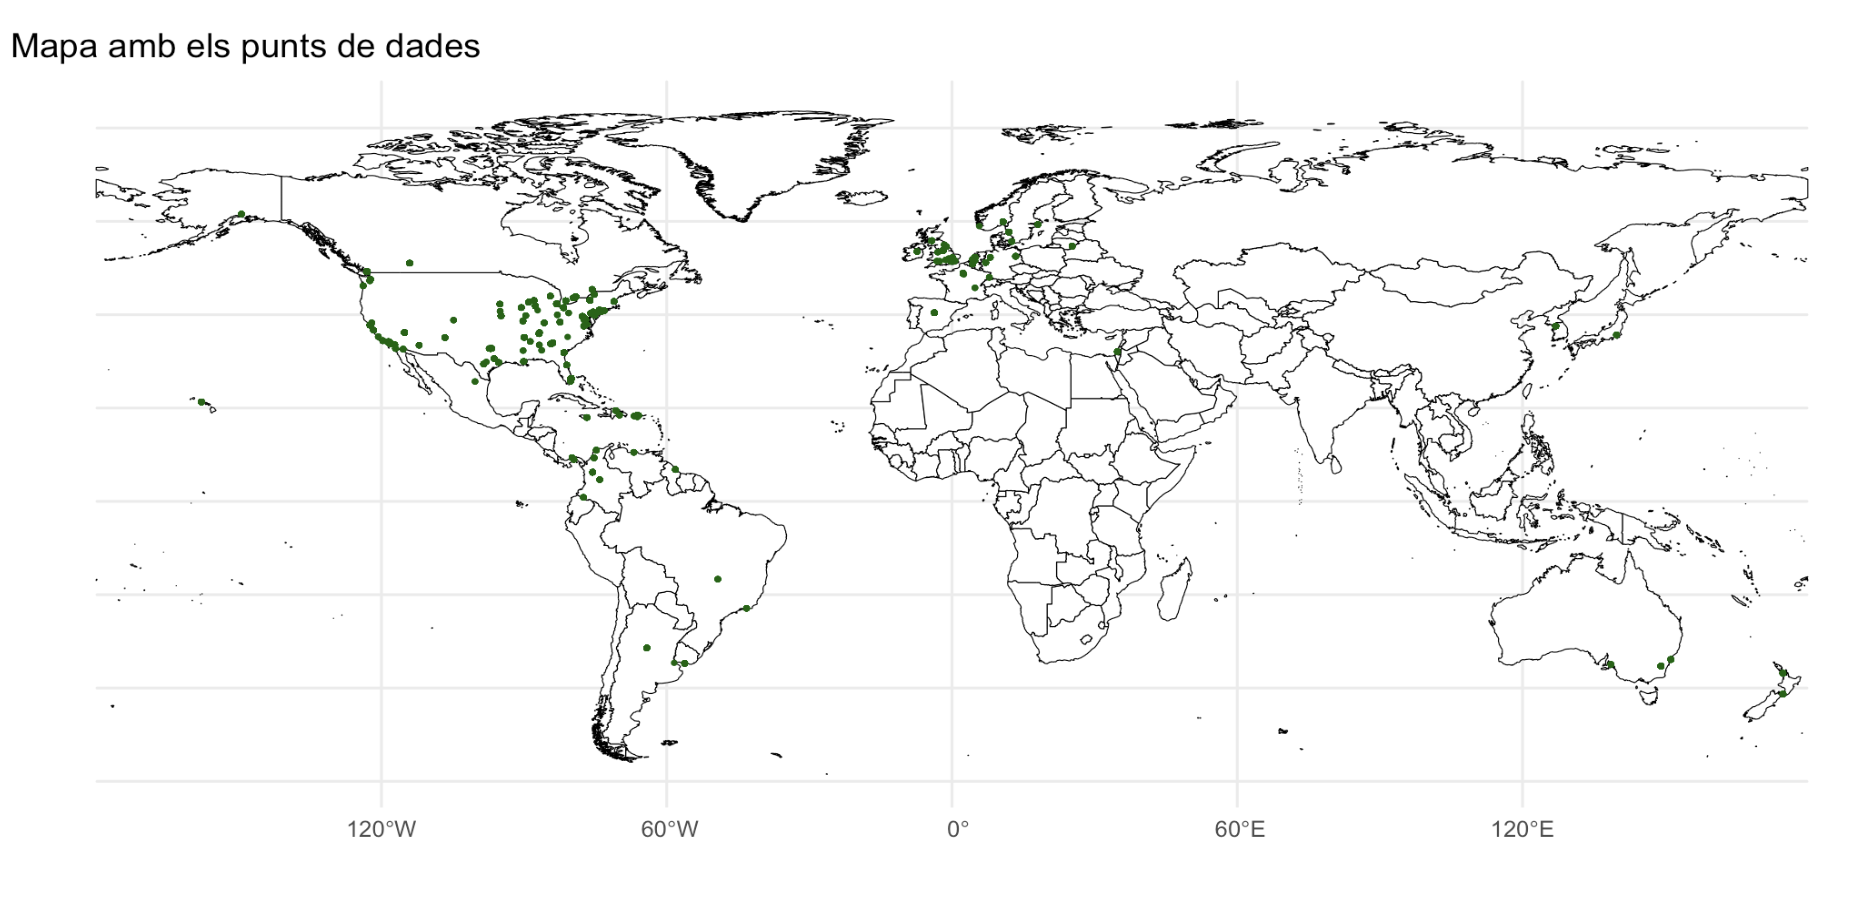
\includegraphics[width=0.7\linewidth]{Images/7_Geospatial/1_descriptive/mapa_punts.png}
    \caption{Mapa amb la ubicació de tots els artistes}
    \label{fig:geo_mapa_punts}
\end{figure}

\begin{figure}[H]
    \centering
    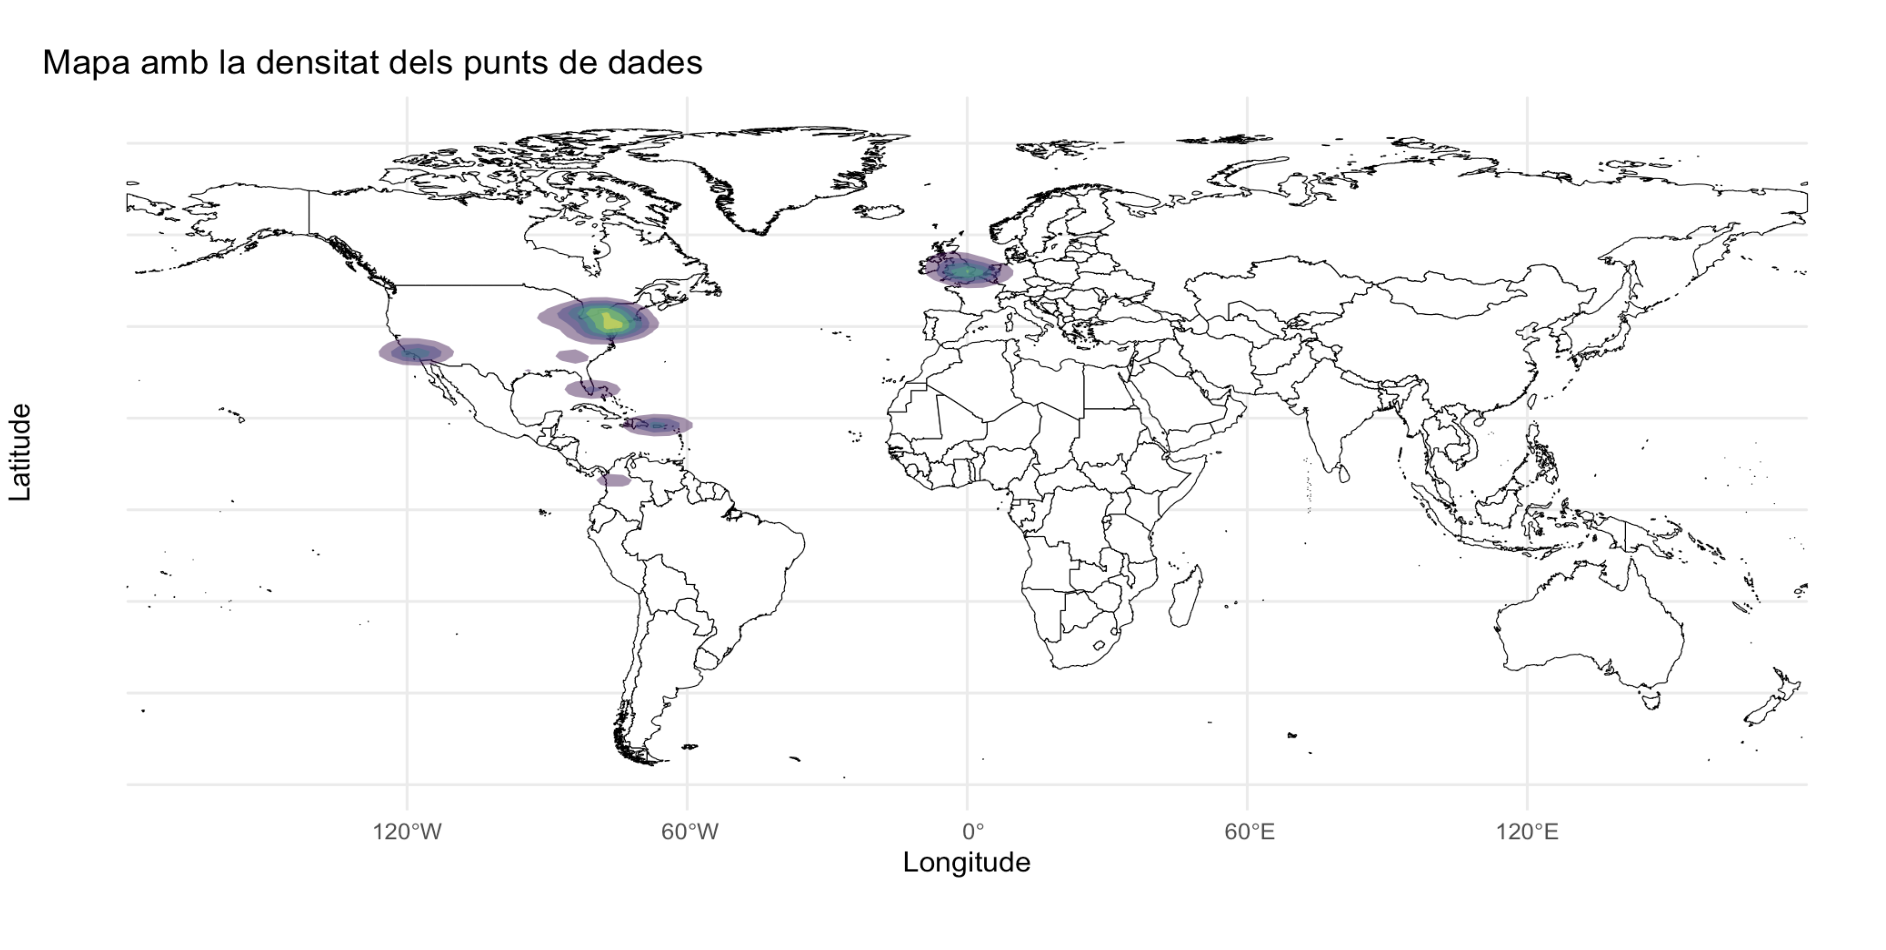
\includegraphics[width=0.7\linewidth]{Images/7_Geospatial/1_descriptive/mapa_intensitat_punts.png}
    \caption{Mapa de densitat dels punts}
    \label{fig:geo_mapa_den}
\end{figure}

Com podem veure, els artistes de les cançons més populars de Spotify venen la seva majoria dels Estats Units, d'Europa i una mica de centre i sud Amèrica. Per això, s'ha fet un plot que visualitza la densitat de punts només de EEUU \ref{fig:geo_mapa_den_eua}. \\

\begin{figure}[H]
    \centering
    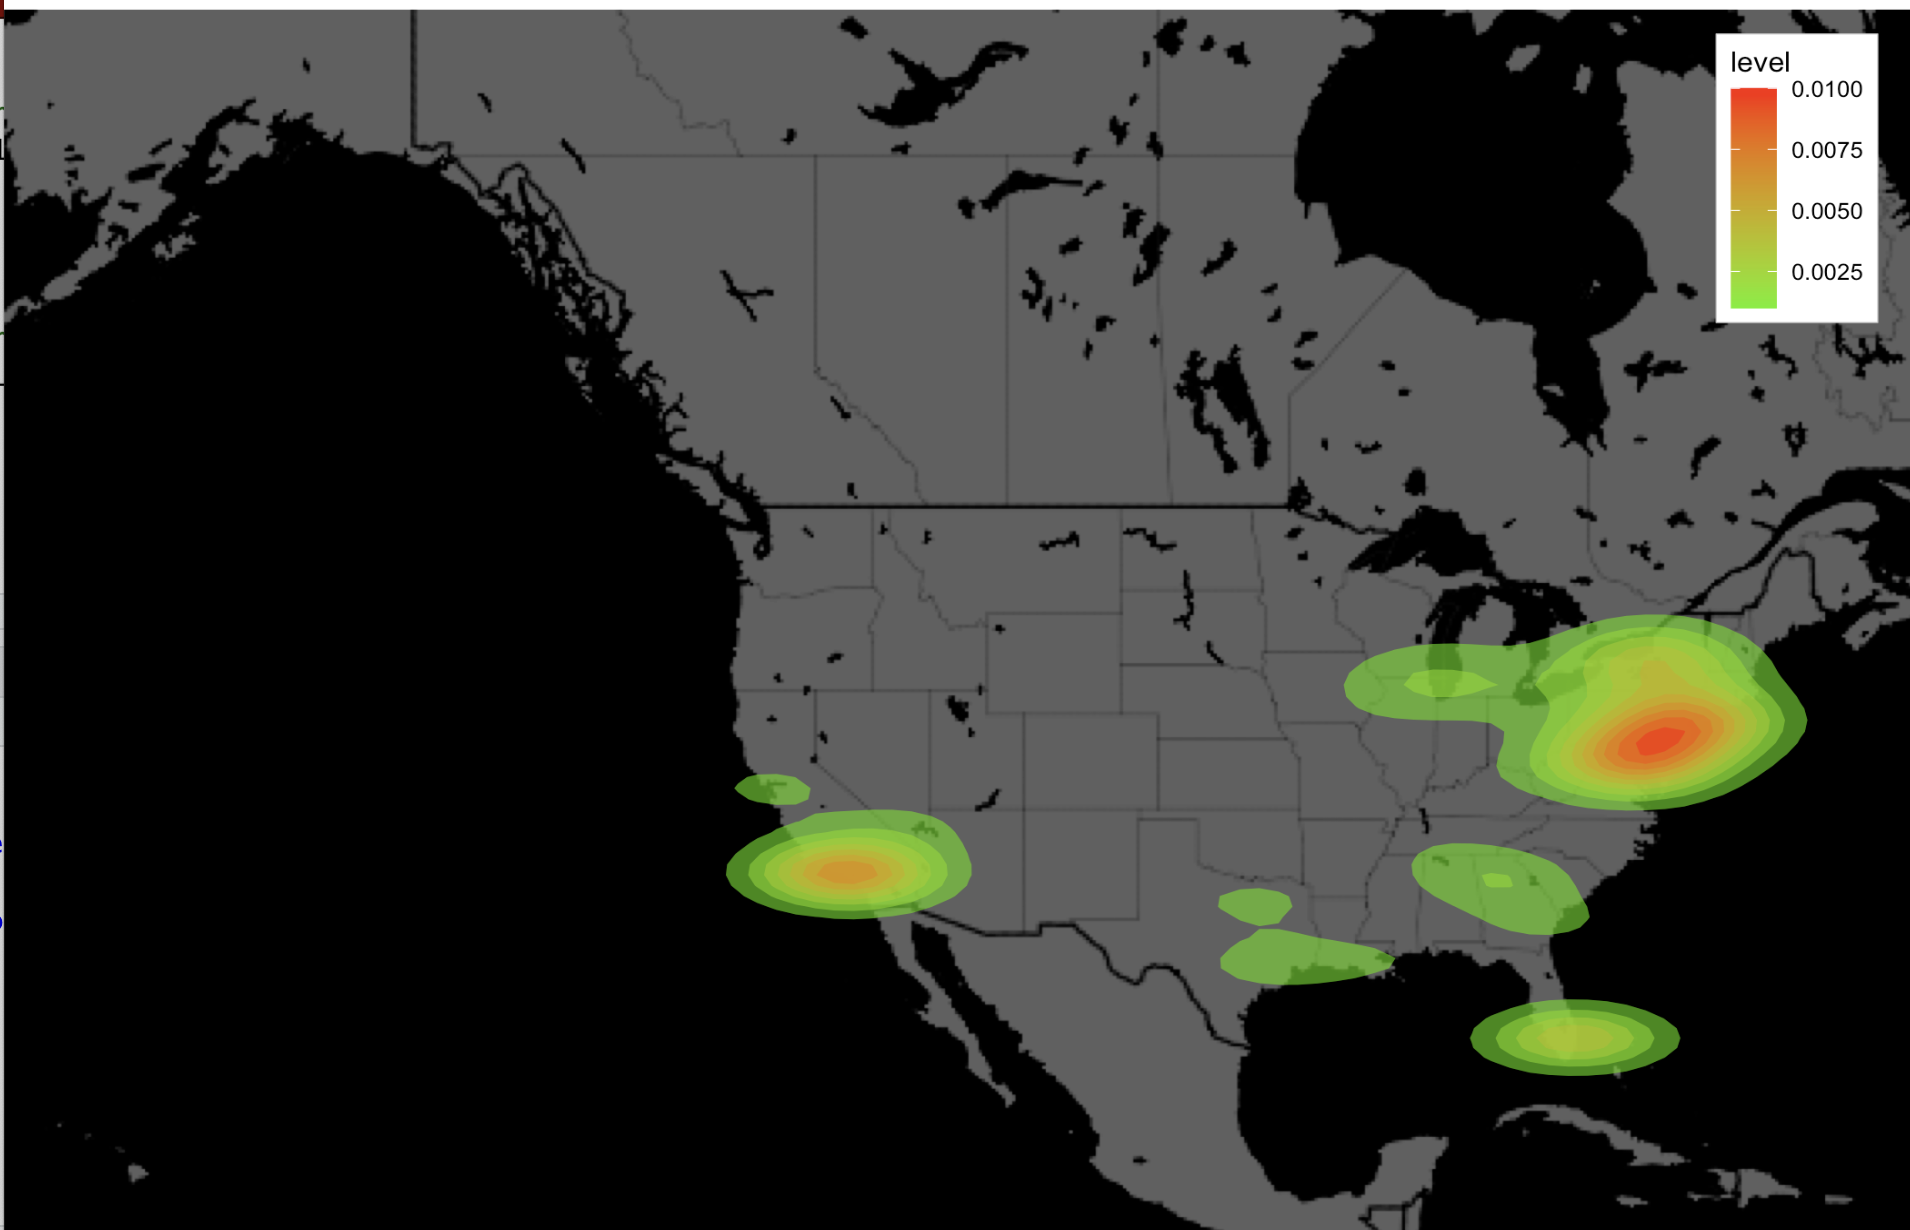
\includegraphics[width=0.6\linewidth]{Images/7_Geospatial/1_descriptive/mapa_densitat_eeuu.png}
    \caption{Mapa de densitat de les cançons a Estats Units}
    \label{fig:geo_mapa_den_eua}
\end{figure}

Veiem al mapa que les zones amb més densitat estan marcades en vermell. Una gran part dels artistes es troben a San Francisco i Los Angeles (Costa Oest). Aquestes regions són molt conegudes per ser centres de la indústria de l'entreteniment. La presència de molts artistes aquí pot estar relacionada amb l'accés a recursos com estudis d'enregistrament, productors musicals... Un altre gran centre que veiem el mapa és Nova York (que es troba a la Costa Est dels EUA). Nova York és una ciutat molt poblada on hi ha molts locals per fer actuacions i també moltes oportunitats pels artistes. Finalment, ha emergit com a centre la ciutat de Houston, Texas. D'aquí han sortit artistes de rap i hip\_hop.\\

D'aquí podem concloure que les grans metròpolis ofereixen grans oportunitats als artistes per poder assolir èxit a Spotify, ja que tenen majors recursos, i hi ha més accessibilitat a professionals del sector, a més de tenir una gran base de consumidors en ser ciutats grans. Podem concloure que els artistes que viuen a aquests centres tenen millors possibilitats de fer-se notar en l'àmbit nacional i internacional. \\

Un exemple pràctic de per què pot ser útil la nostra anàlisi, són els artistes emergents. Si un artista vol donar-se a conèixer, ha de saber que és crucial residir o connectar-se amb gent d'aquests llocs i així tenir èxit a Spotify. També pot ser útil per una ciutat que vol fomentar la seva pròpia escena musical, que llavors haurà d'invertir en infraestructures que suportin els artistes locals. \\

% també posar una altra com energy o algo així

\begin{figure}[H]
    \centering
    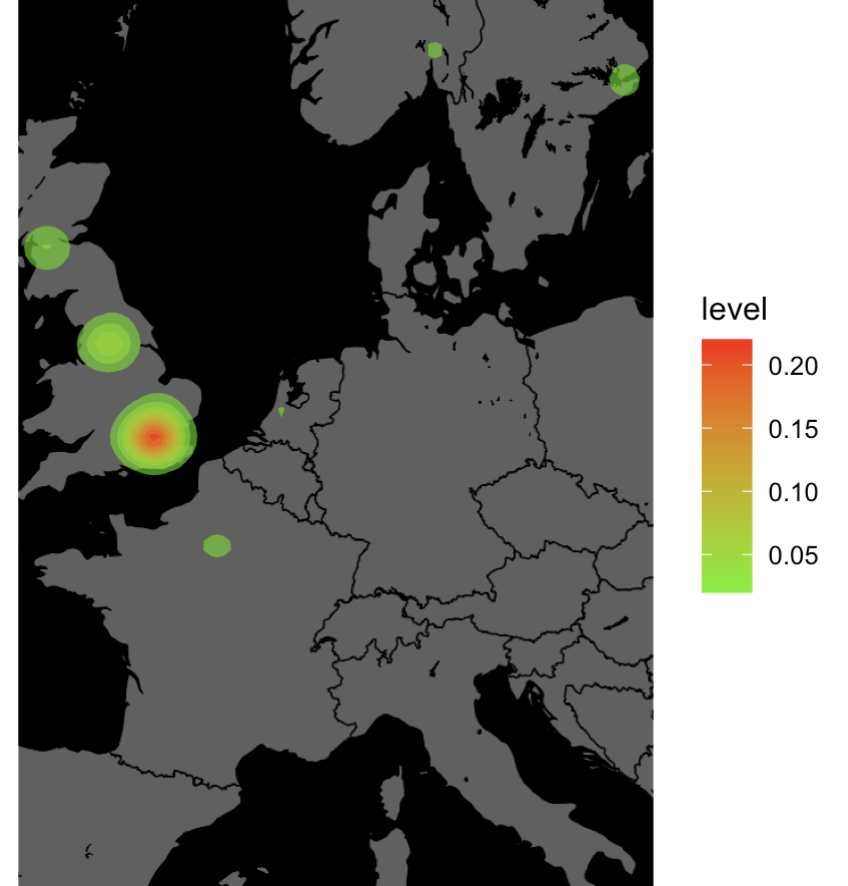
\includegraphics[width=0.4\linewidth]{Images/7_Geospatial/1_descriptive/mapa_densitat_europa.png}
    \caption{Mapa de densitat de les cançons a Europa}
    \label{fig:geo_mapa_den_europa}
\end{figure}

També sabem que un dels llocs on més es veu concentració de cançons és Regne Unit, pel mapa \ref{fig:geo_mapa_den_europa} ja veiem clar que Londres és el lloc amb més cançons famoses d'artistes. Tot i això, també hi ha un centre a Halifax i un altre a Glasgow. Si en comptes de mirar la freqüència de mostres, mirem la freqüència, però filtrant perquè només surti un cop cada artista o només surti un cop capa cançó de cada artista, veiem que a Halifax i Glasgow només tenen un artista del top. Aquests són Ed Sheeran i Lewis Capaldi, que han estat tantes setmanes en el top, i en el cas d'Ed Sheeran amb tantes cançons diferents, que es forma una zona amb densitat. A continuació podem veure un mapa una mica més acurat amb la freqüència però d'artistes i no de cançons. \\

Un cop hem visualitzat tots els punts al mapa, farem una sèrie de plots per observar si les característiques dels artistes i les seves cançons depenen del lloc d'on venen o no. Com hi ha una gran majoria de punts concentrats en els mateixos països (EUA i Regne Unit com s'ha visualitzat anteriorment), és molt probable que no puguem extreure gaire informació, però sí que es poden extreure conclusions dels països on hi ha menys representació d'artistes, ja que hi ha menys varietat.

\begin{figure}[H]
    \centering
    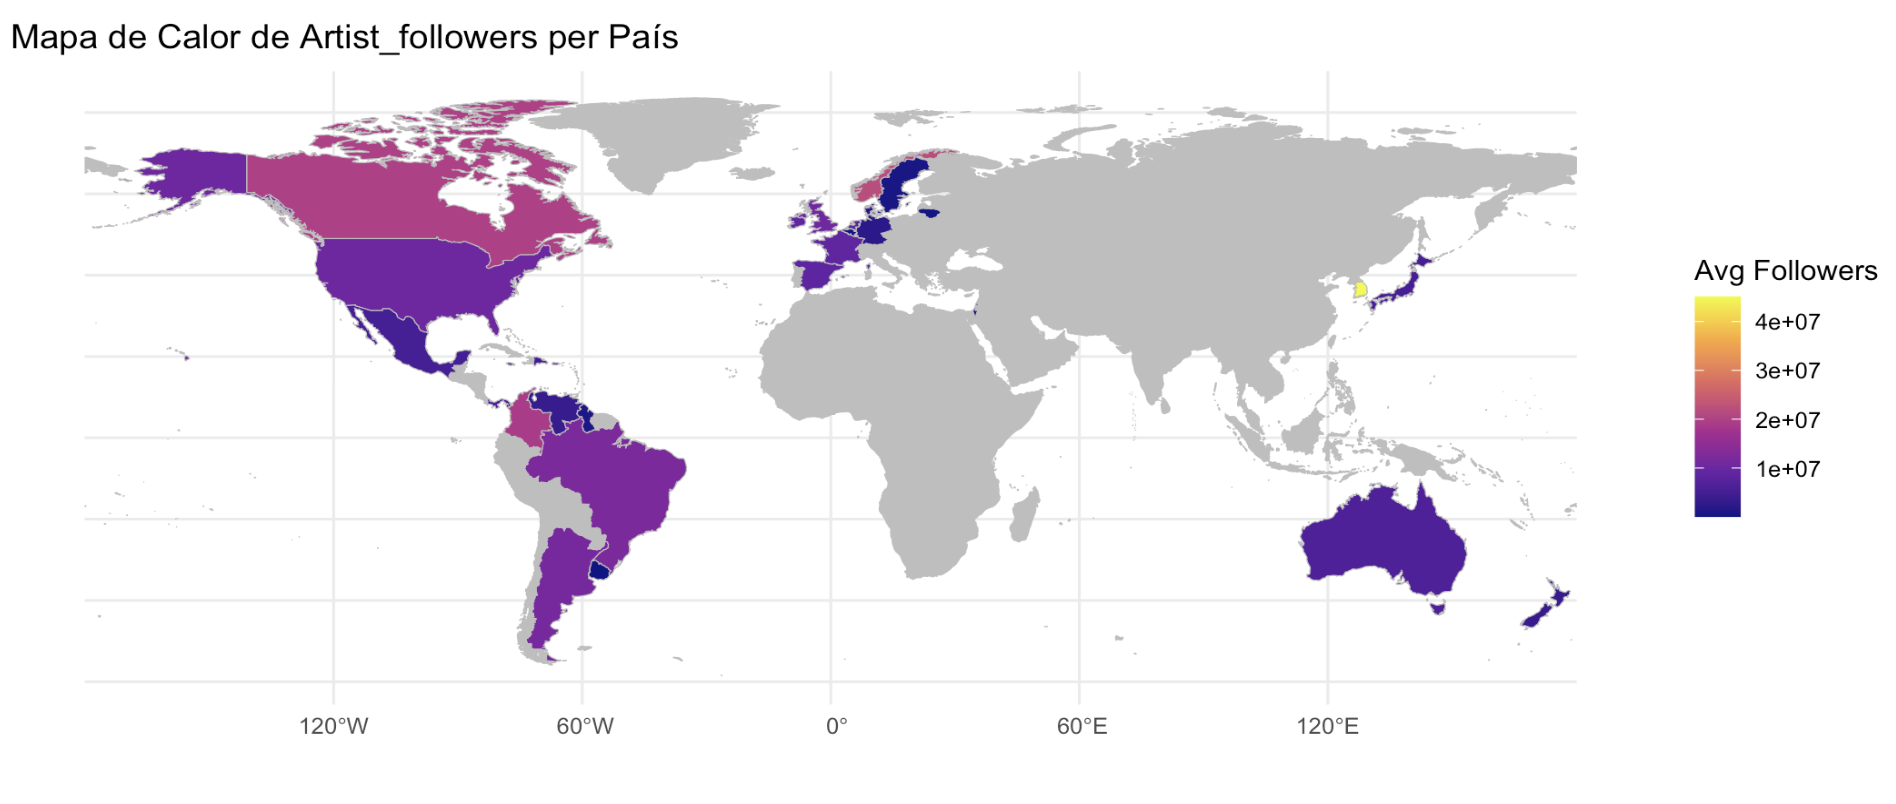
\includegraphics[width=0.8\linewidth]{Images/7_Geospatial/1_descriptive/mapa_artist_followers.png}
    \caption{Mitjana de followers dels artistes de cada país}
    \label{fig:geo_mean_follow}
\end{figure}

En la Figura \ref{fig:geo_mean_follow} podem veure les mitjanes de quants seguidors tenen els artistes a cada país. S'ha de tenir en compte que tots aquests artistes han passat pel Top de Spotify aleshores la gran majoria tenen molts seguidors. Veiem que els països on hi ha menys cançons, com per exemple, Finlàndia o Alemanya, són els països on els artistes tenen menys seguidors (amb un color lila tirant a blau). L'excepció d'això és Corea del Sud, que veiem que és l'únic país groc (amb una mitjana de més de 4 milions). Això és pel fet que els pocs artistes que provenen d'allà (sabem que són BTS i BlackPink) han tingut molta influència aquests anys i, per tant, compten amb molts seguidors. Contràriament a això, els països que disposen de molts artistes en el top, com són els Estats Units i el Regne Unit, tenen una mitjana de followers més baixa, ja que tenen una varietat d'artistes que tenen diferents nivells de seguidors.

A més de visualitzar si els valors de les nostres dades variaven segons el país o la ciutat segons d'on és l'artista, ara també volem veure si la variable temporal té alguna influència. En el següent plot observem els valors mitjans dels seguidors dels artistes per país, i també per cada any \ref{fig:geo_mean_year_follow}.

\begin{figure}[H]
    \centering
    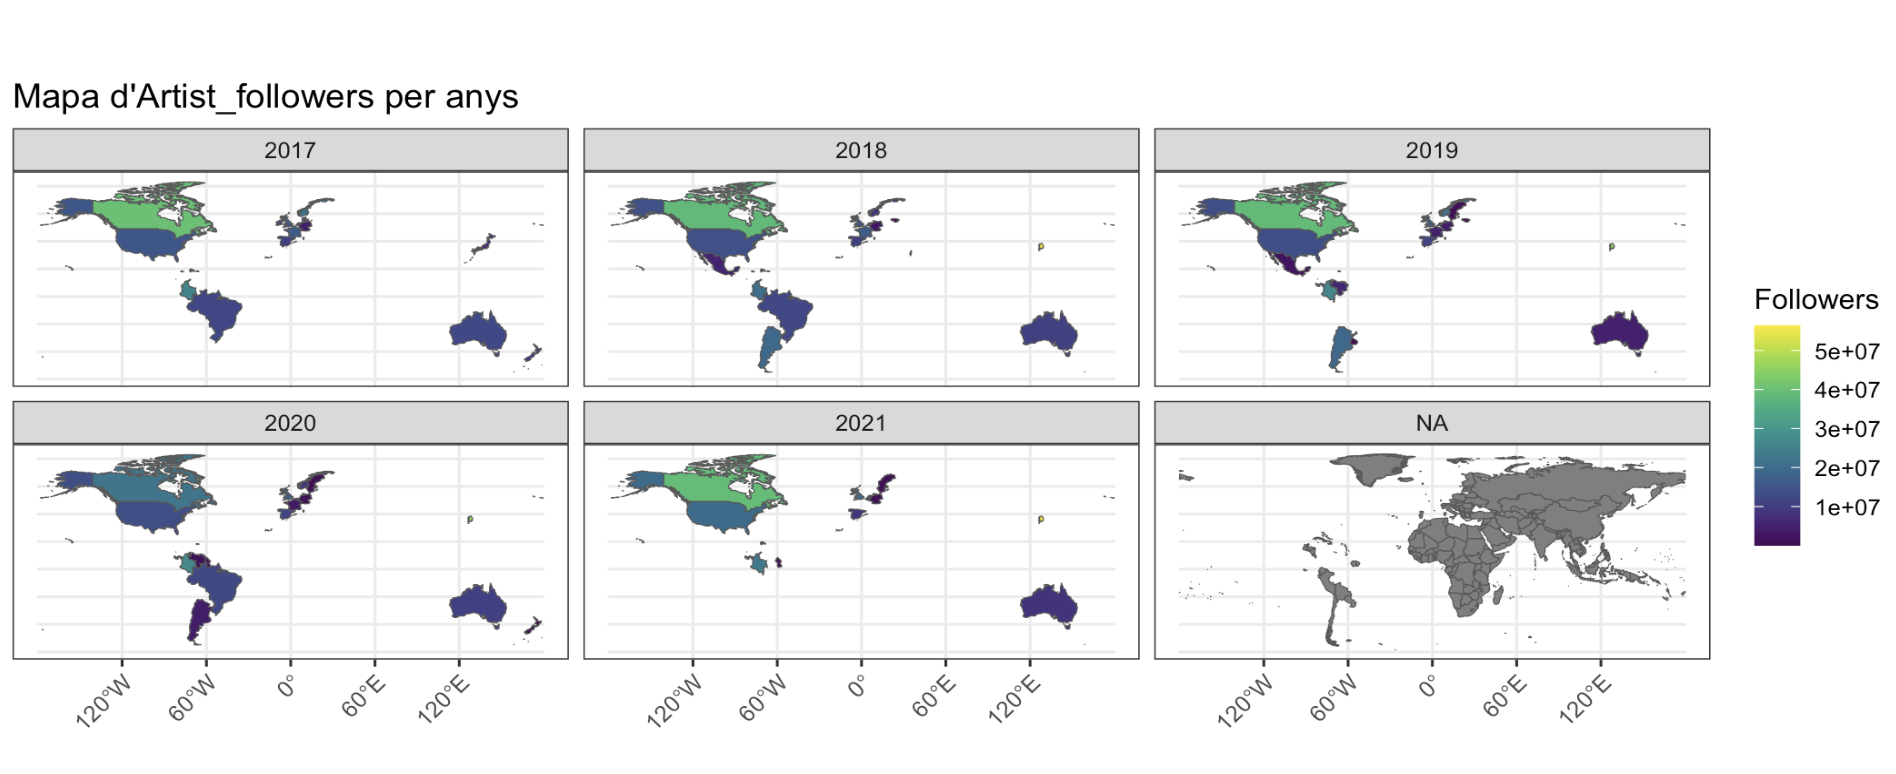
\includegraphics[width=0.8\linewidth]{Images/7_Geospatial/1_descriptive/mapa_artist_followers_years.png}
    \caption{Mitjana de followers dels artistes de cada país per cada any}
    \label{fig:geo_mean_year_follow}
\end{figure}

Veiem que cada submapa representa un any diferent des de 2017 fins a 2021. S'ha utilitzat la variable year\_week per fer aquesta visualització, ja que ens diu l'any en el qual va sortir cada cançó al top. Si haguéssim utilitzat la variable year\_release, tindríem anys de més anys, perquè hi ha cançons antigues que en algun moment han tornat a ser populars aquests 5 anys. En el sisè mapa, hi trobem els països que no han sortit mai en el top que són marcats com a NA. La resta de mapes utilitzen una escapa de colors per indicar el nombre de seguidors, que variable des de menys d'un milió fins a més de 50 milions. \\

Si observem la Figura, veiem que els anys entre 2017 i 2019 tenen la mateixa tendència, on hi ha una concentració d'artistes amb molts seguidors a Nord-amèrica, i això es manté contant al llarg dels tres anys. Europa també mostra un nivell alt de seguidors. L'Amèrica del Sud, especialment el Brasil, destaca igualment durant aquests anys. \\

L'any 2020, es pot observar un augment en la densitat de seguidors a Austràlia, la qual cosa pot indicar un creixement en la popularitat de certs artistes en aquesta regió.
Nord-amèrica i Europa mantenen una presència forta, amb una densitat lleugerament augmentada en comparació amb els anys anteriors. \\

L'any 2021, hi ha un augment notable en la concentració de seguidors a parts de l'Àsia, particularment a l'Índia i l'Àsia Oriental. Aquest canvi pot reflectir l'expansió de plataformes com Spotify en nous mercats durant aquest període. Els patrons de densitat a Europa i Nord-amèrica semblen constants, amb una presència lleugerament augmentada en comparació amb els anys anteriors.

Les conclusions que podem extreure de relacionar la nostra variable temporal amb la geoespacial, és que hi ha hagut una expansió a regions com Austràlia i l'Àsia en els últims anys. Això podria indicar que s'han esforçat per connectar amb nous públics i gràcies a l'augment d'ús de plataformes digitals hi ha hagut una globalització musical. També concloem que en general el que més es manté en el top són artistes dels Estats Units, i també europeu, ja que ja estan consolidats a la indústria musical. Els artistes i les empreses de la indústria poden utilitzar aquesta informació per a orientar millor els seus esforços de màrqueting i expansió en diferents regions.\\

Després es realitzarà una modelització i una predicció d'algunes variables segons la seva localització, per això, a part de la popularitat dels artistes veurem l'energia de les cançons.

Després d'observar la distribució geoespacial i temporal de variables numèriques, també hem volgut veure el comportament de les nostres variables categòriques als diferents països. Volem veure si hi ha diferències entre els gèneres musicals que canten els artistes de diferents països i si hi ha diferències també en l'ús de col·laboracions o paraules explícites. Pot ser interessant veure si la identitat cultural de cada un dels països es veu reflectida en la seva música. A més, analitzar les lletres explícites dels països pot reflectir també les condicions socials i polítiques d'aquell país.

Saber els gèneres més fets per cada país és extremadament interessant, ja que està molt relacionat amb les característiques dels artistes. Per això, a la següent figura podem veure quin és el gènere més fet a cada país \ref{fig:geo_genres_country}.
% plot gèneres i collab i explicit
\begin{figure}[H]
    \centering
    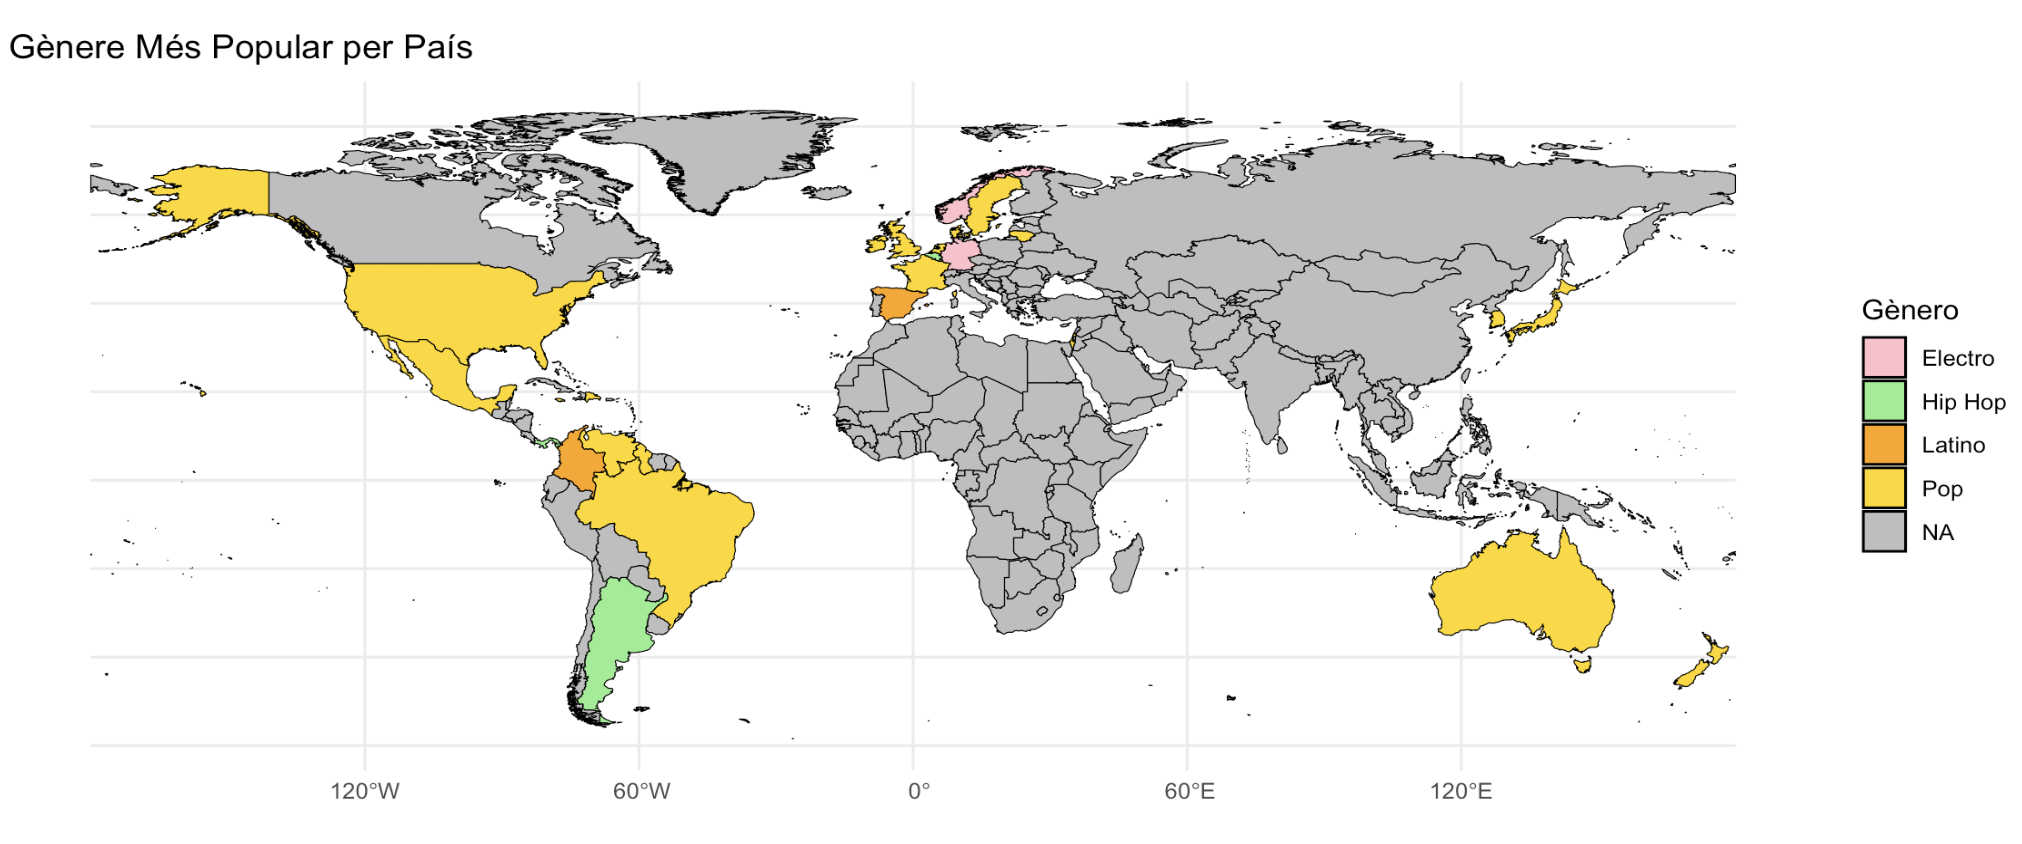
\includegraphics[width=0.8\linewidth]{Images/7_Geospatial/1_descriptive/genere_mes_popular_per_pais.png}
    \caption{Gènere més popular de cada país}
    \label{fig:geo_genres_country}
\end{figure}

Com podem veure, a la majoria dels països predomina el Pop, això és degut al fet que una gran majoria de les nostres mostres són de Pop i molts cops les cançons d'altres gèneres són una barreja entre pop i altres, aleshores hi ha moltes mostres de pop. Veiem que només hi ha dos països, Espanya i Colòmbia, que generem com a més populars cançons de Latino, té sentit, ja que són països hispanoparlants. També veiem que Alemanya i Noruega generen molt electro. Aquestes dades fan sentit perquè Alemanya des dels anys 70 ha estat lloc on més DJs i de música electrònica es fa. Finalment, l'Hip-hop guanya a Argentina.

Per entrar més profundament en els següents plots visualitzarem el percentatge de cançons que surten de cada gènere per cada país.

\begin{figure}[H]
\centering
    \begin{minipage}{.5\textwidth}
        \centering
        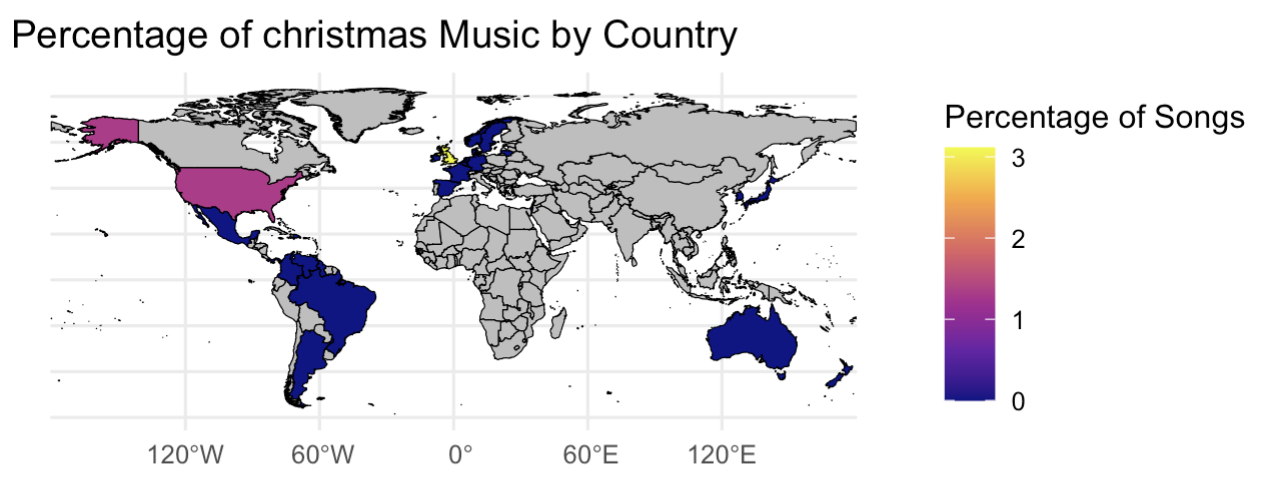
\includegraphics[width=0.99\linewidth]{Images/7_Geospatial/1_descriptive/percent_genere_per_pais/per_christmas.png}
        \caption{Mapa del percentatge de Christmas}
        \label{fig:geo_christmas_country}
    \end{minipage}%
    \begin{minipage}{.5\textwidth}
        \centering
        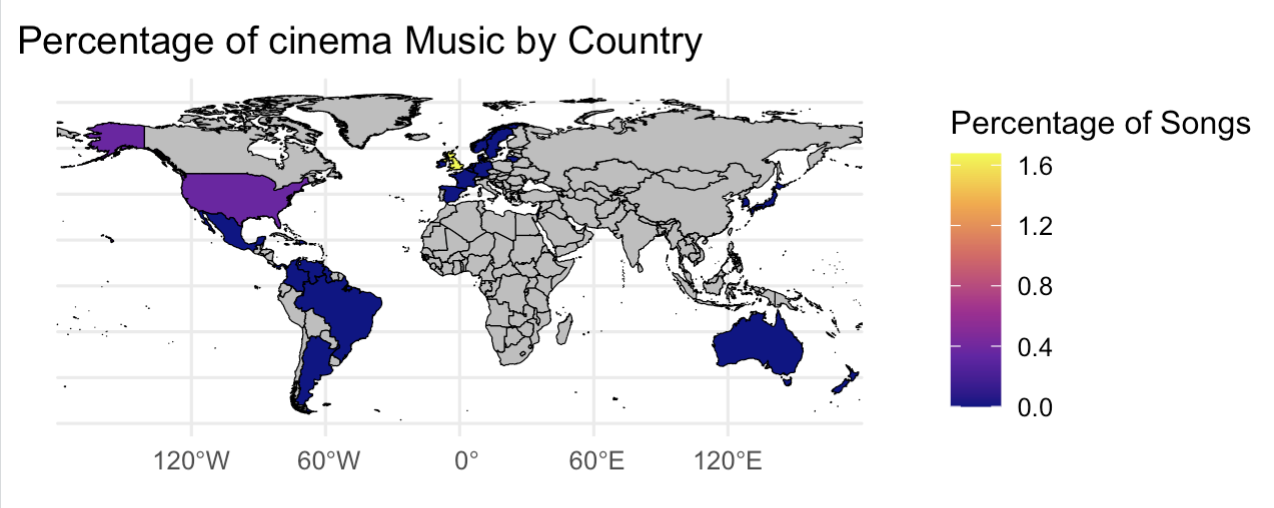
\includegraphics[width=0.99\linewidth]{Images/7_Geospatial/1_descriptive/percent_genere_per_pais/per_cinema.png}
        \caption{Mitjana del percentatge de Cinema}
        \label{fig:geo_cinema_country}
    \end{minipage}%
\end{figure}

Primer de tot veiem el gènere Cinema \ref{fig:geo_cinema_country}, que apareix amb un màxim d'un 2\% a Regne Unit i també als Estats Units. Això és pel fet que ambdues tenen indústries cinematogràfiques molt influents globalment (Hollywood per exemple). Aquestes no només generem moltes pel·lícules, sinó també tenen una distribució internacional significativa, cosa que augmenta l'exposició de les seves bandes sonores. \\
En el cas de les cançons de Christmas, \ref{fig:geo_christmas_country}, passa el mateix perquè només hi ha cançons de Christmas en anglès i, per tant, venen d'aquests països.

\begin{figure}[H]
\centering
    \begin{minipage}{.5\textwidth}
        \centering
        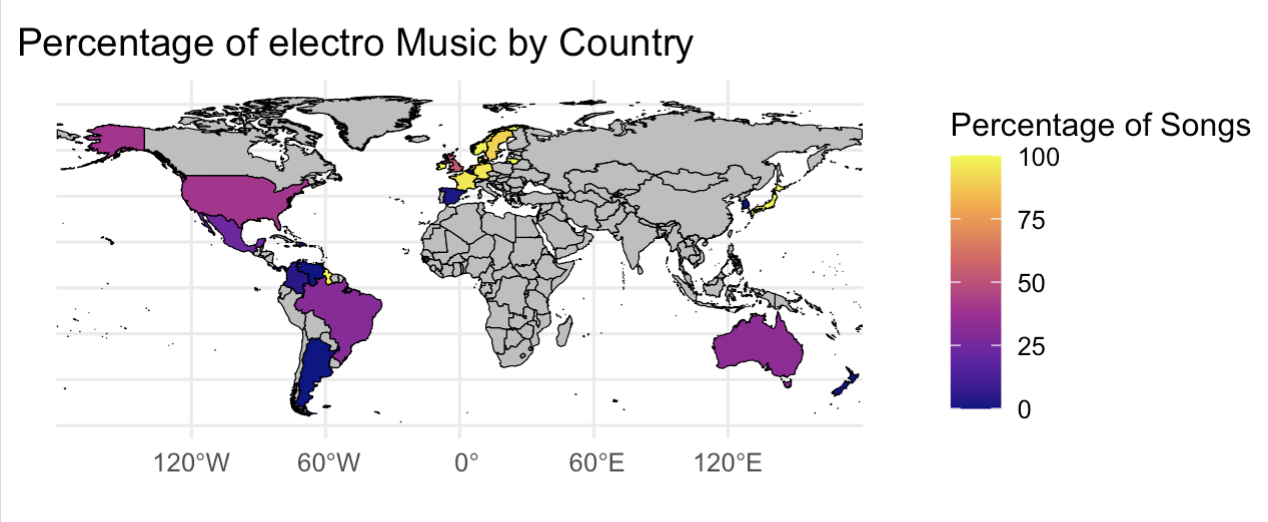
\includegraphics[width=0.99\linewidth]{Images/7_Geospatial/1_descriptive/percent_genere_per_pais/per_electro.png}
        \caption{Mapa del percentatge de Electro}
        \label{fig:geo_electro_country}
    \end{minipage}%
    \begin{minipage}{.5\textwidth}
        \centering
        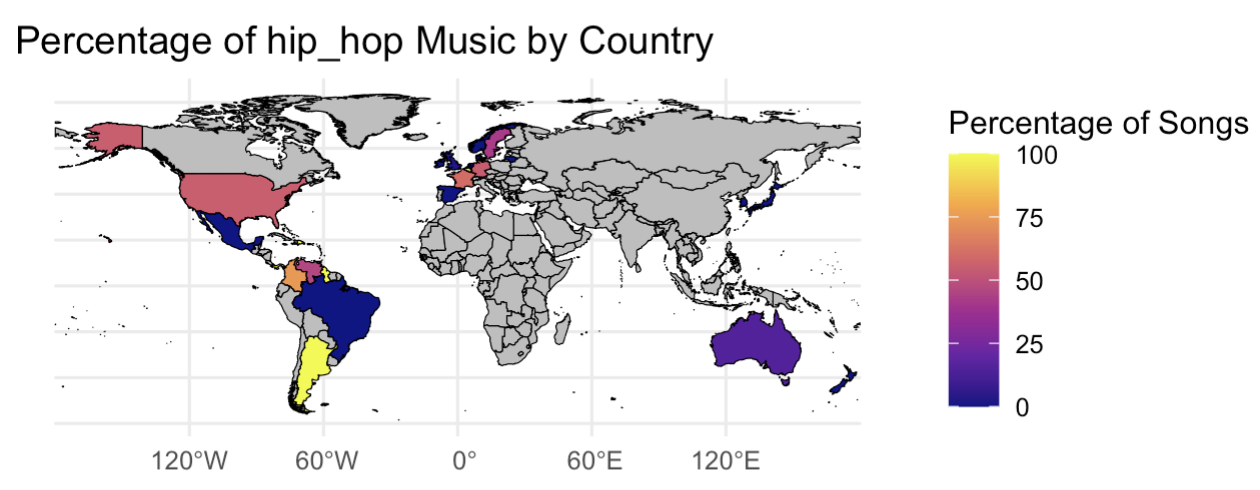
\includegraphics[width=0.99\linewidth]{Images/7_Geospatial/1_descriptive/percent_genere_per_pais/per_hiphop.png}
        \caption{Mitjana del percentatge de Hip\_Hop}
        \label{fig:geo_hiphop_country}
    \end{minipage}%
\end{figure}
A continuació veiem la música electrònica,\ref{fig:geo_electro_country}, que com hem vist actualment, té un alt percentatge als països nòrdics i sobretot a Alemanya. El que sorprèn és que també hi ha un alt percentatge a França, cosa que no havia sortit en els plots anteriors. Pels altres països hi ha un percentatge més baix tot i que no és inexistent. \\

Veiem que la distribució canvia en el cas del Hip-hop \ref{fig:geo_hiphop_country}. Els Estats Units té més d'un 50\% de cançons de hip-hop i també a Europa hi ha molta representació. El que més sorprèn és que a Argentina hi ha el percentatge més alt, que segurament és degut a una barreja amb altres gèneres i també es pot relacionar amb els nivells de \textit{speechiness} anterior.

\begin{figure}[H]
\centering
    \begin{minipage}{.5\textwidth}
        \centering
        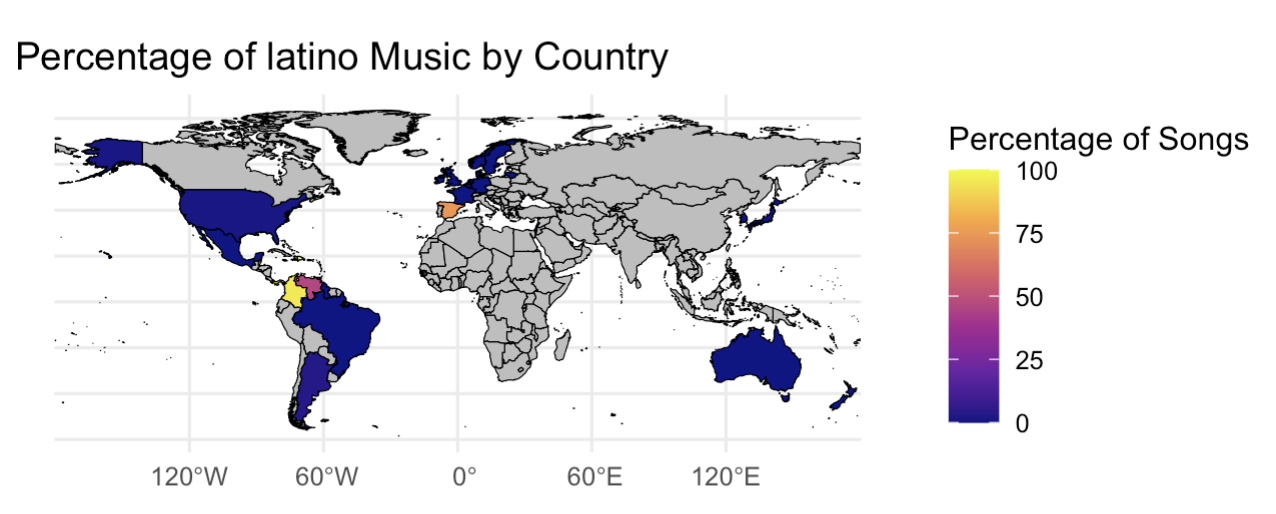
\includegraphics[width=0.99\linewidth]{Images/7_Geospatial/1_descriptive/percent_genere_per_pais/per_latino.png}
        \caption{Mapa del percentatge de Latino}
        \label{fig:geo_latino_country}
    \end{minipage}%
    \begin{minipage}{.5\textwidth}
        \centering
        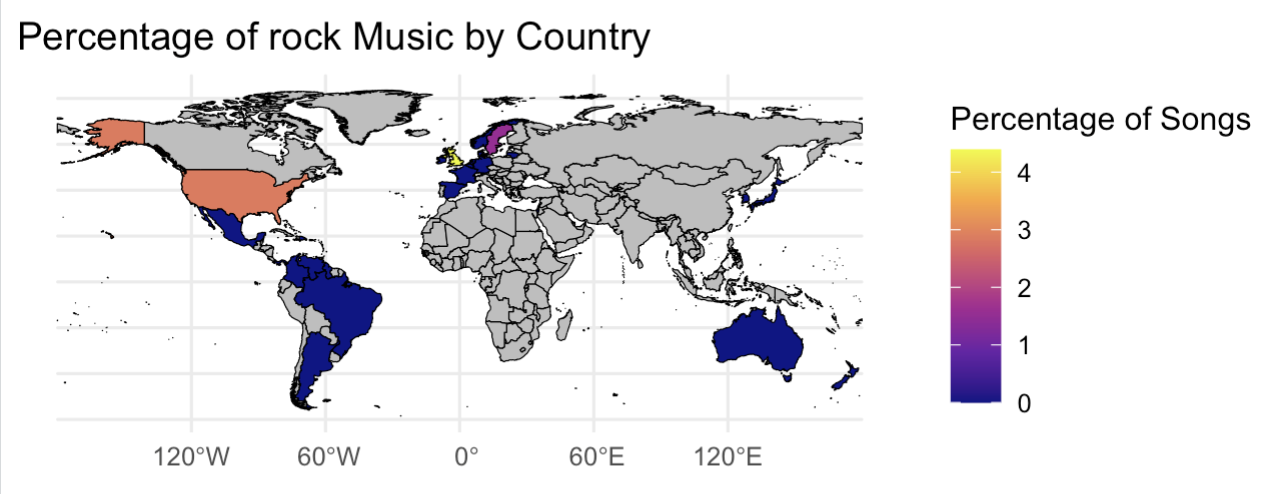
\includegraphics[width=0.99\linewidth]{Images/7_Geospatial/1_descriptive/percent_genere_per_pais/per_rock.png}
        \caption{Mitjana del percentatge de Rock}
        \label{fig:geo_rock_country}
    \end{minipage}%
\end{figure}

Com hem vist al plot de tots els gèneres, els països amb un percentatge més alt de cançons de latino és a Espanya i a Centreamèrica. Als altres països el percentatge és molt proper a zero, cosa que vol dir que és un gènere que es fa exclusivament a aquests països \ref{fig:geo_latino_country}. \\

Després tenim un altre gènere, rock \ref{fig:geo_rock_country}, que compta amb poques cançons i només està als Estats Units, a Regne Unit, i a algun altre país europeu, i estan també combinats amb el gènere pop.

\begin{figure}[H]
\centering
    \begin{minipage}{.5\textwidth}
        \centering
        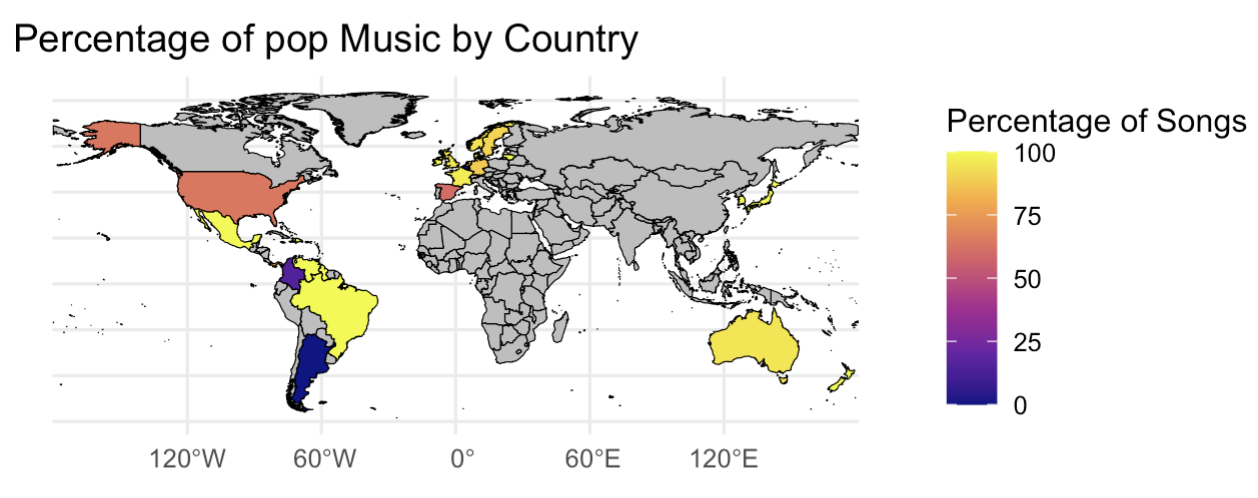
\includegraphics[width=0.99\linewidth]{Images/7_Geospatial/1_descriptive/percent_genere_per_pais/per_pop.png}
        \caption{Mapa del percentatge de Pop}
        \label{fig:geo_pop_country}
    \end{minipage}%
    \begin{minipage}{.5\textwidth}
        \centering
        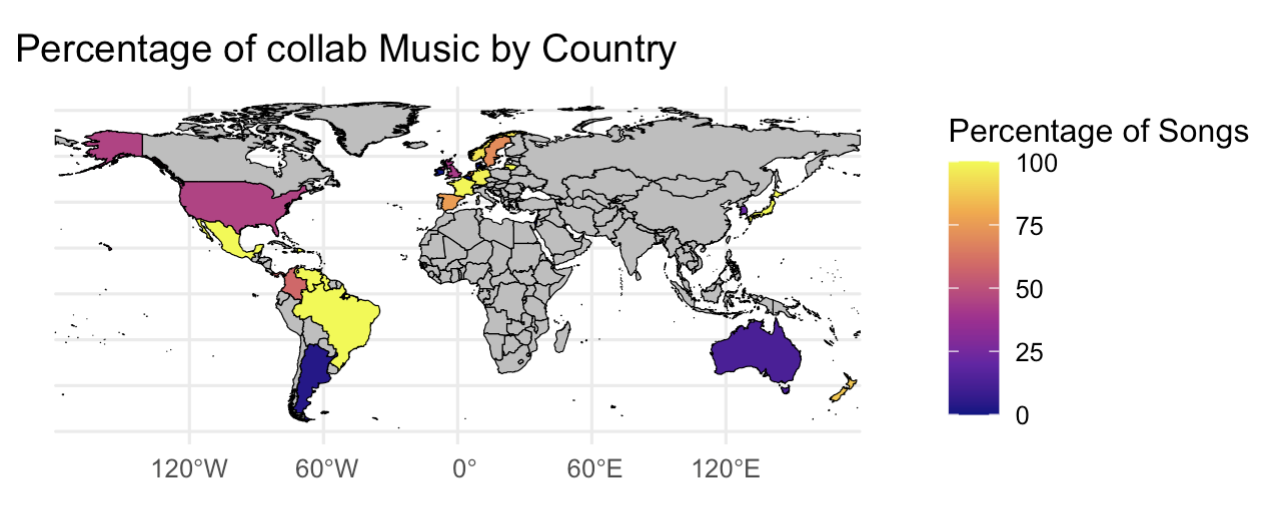
\includegraphics[width=0.99\linewidth]{Images/7_Geospatial/1_descriptive/percent_genere_per_pais/per_collab.png}
        \caption{Mitjana del percentatge de Collab}
        \label{fig:geo_collab_country}
    \end{minipage}%
\end{figure}

Finalment, tenim el plot pel Pop \ref{fig:geo_pop_country}, que veiem òbviament tenen els percentatges més alts, menys a Argentina i a Colòmbia, on predominàvem altres gèneres. Com s'ha comentat, el pop és molt propens a ser combinat amb altres gèneres, per tant, apareix a la gran majoria de les cançons. \\

També hem considerat interessant visualitzar altres variables categòriques, com collab. Concloem que Austràlia és el país on menys col·laboracions hi ha. En canvi, al Brasil, Mèxic, i Alemanya gairebé el 100\% són col·laboracions. Això es pot deure al fet que el tipus de cançons que es fan a aquests països (electro per Alemanya, o Latino a Mèxic) solen tenir moltes col·laboracions.

% Mapes interactius

A part de fer una anàlisi de les dades en el mapa estàtic, també s'ha fet un mapa interactiu on no només es poden veure tots els diferents punts al mapa, sinó que també se'ls diferencia segons la popularitat de l'artista, els seus followers o el gènere musical més comú de les seves cançons. D'aquesta manera no només veiem les distribucions per països, sinó també veiem les de les ciutats.

\begin{figure}[H]
\centering
    \begin{minipage}{.5\textwidth}
        \centering
        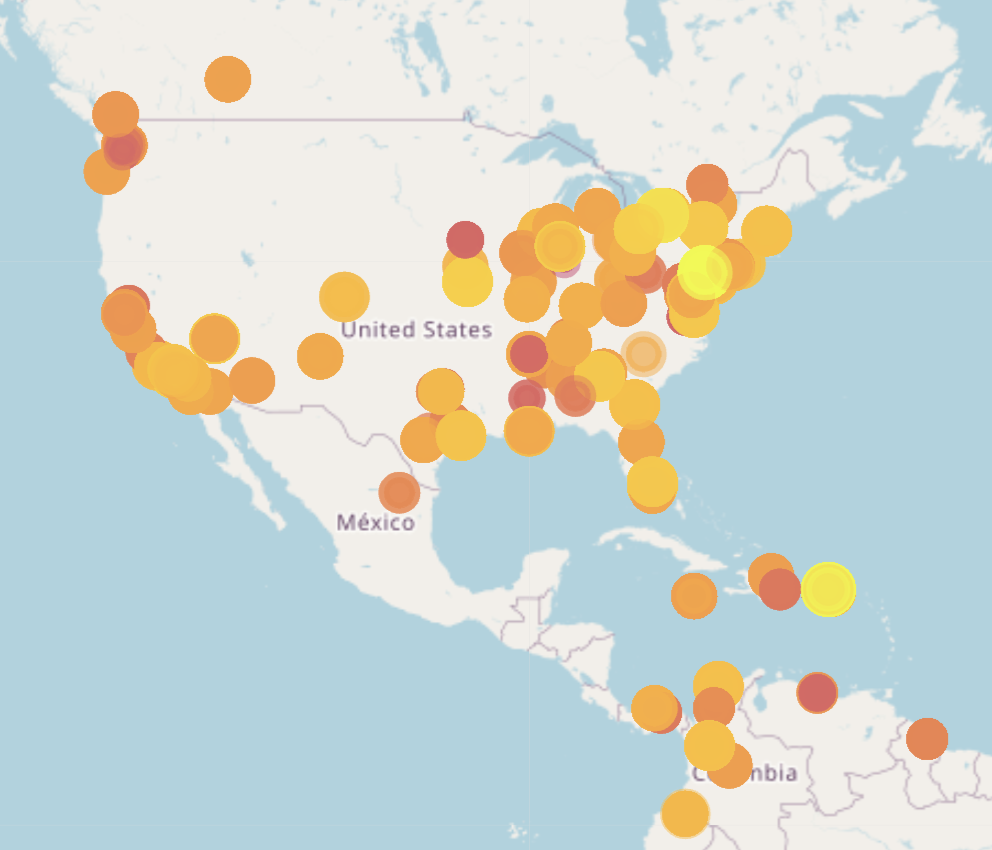
\includegraphics[width=0.99\linewidth]{Images/7_Geospatial/1_descriptive/map_interactiu1.png}
        \caption{Mapa interactiu 1}
        \label{fig:geo_pop_country}
    \end{minipage}%
    \begin{minipage}{.5\textwidth}
        \centering
        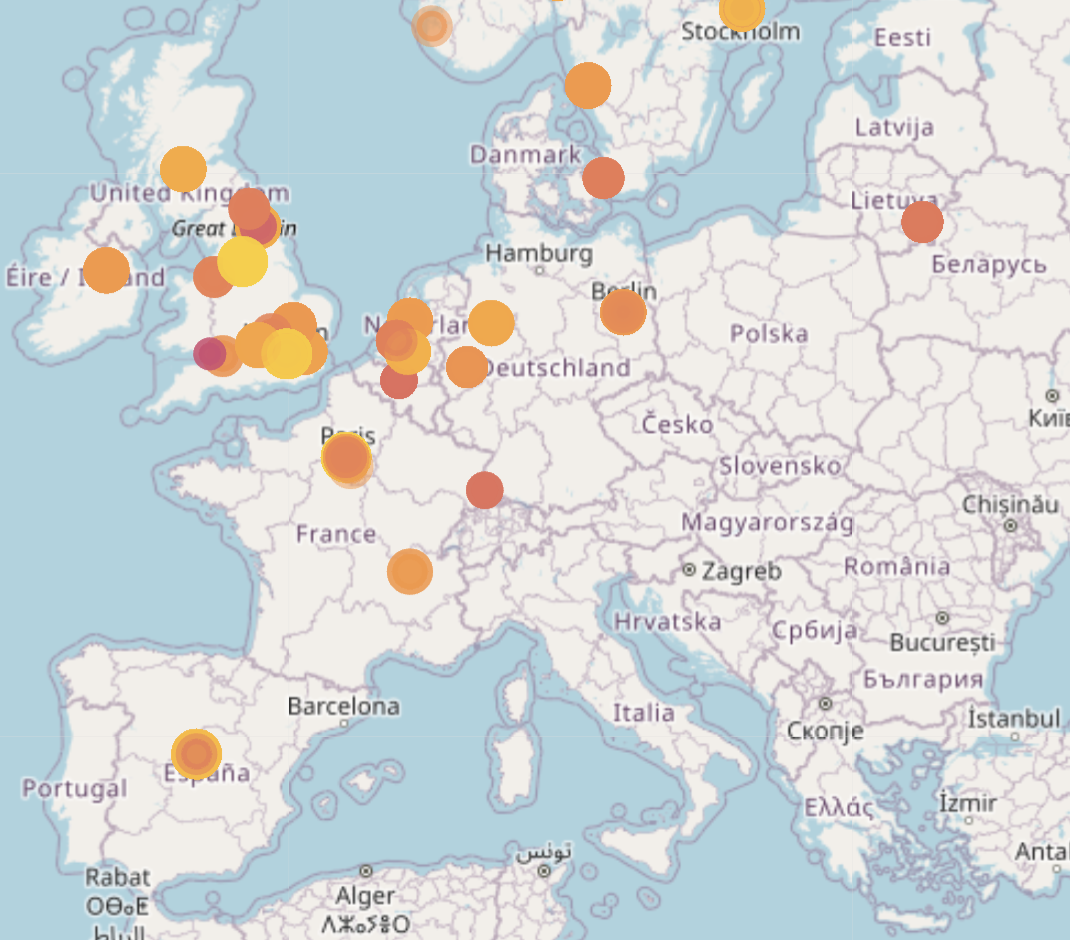
\includegraphics[width=0.99\linewidth]{Images/7_Geospatial/1_descriptive/map_interactiu2.png}
        \caption{Mapa interactiu 2}
        \label{fig:geo_collab_country}
    \end{minipage}%
\end{figure}

%les altres dadesssssss

Després de fer una anàlisi completa de les nostres dades geospacials, com la nostra base de dades comptava amb localitzacions poc variades (tenim molt pocs països), s'ha decidit fer ús d'una nova base de dades per veure les tendències a altres països. \\

Aquesta base de dades comptava originalment amb el TOP 50 de Spotify escoltat per cada país cada dia. Aleshores, disposa de més països que les nostres dades originals i tracta amb dades actuals (no dels anys 2017-2021 amb les que tractàvem anteriorment). Per simplificar la nostra anàlisi s'han fet dos canvis a la database. Primer de tot, s'ha reduït al top 5 cançons de cada dia per cada país. Després, també s'ha creat una altra que és la mitjana del top 50 per cada país, fent la mitjana dels dies i deixant-nos amb una sola mostra de cada país. Treballarem amb aquestes dues bases de dades també per veure si podem extreure conclusions sobre els nous països i sobre el que escolta més cada un dels països.

%%%%%% MEAN
A continuació es fa l'anàlisi descriptiva geospacial de les dades que tenen la mitjana d'aquesta base de dades.

\begin{figure}[H]
    \centering
    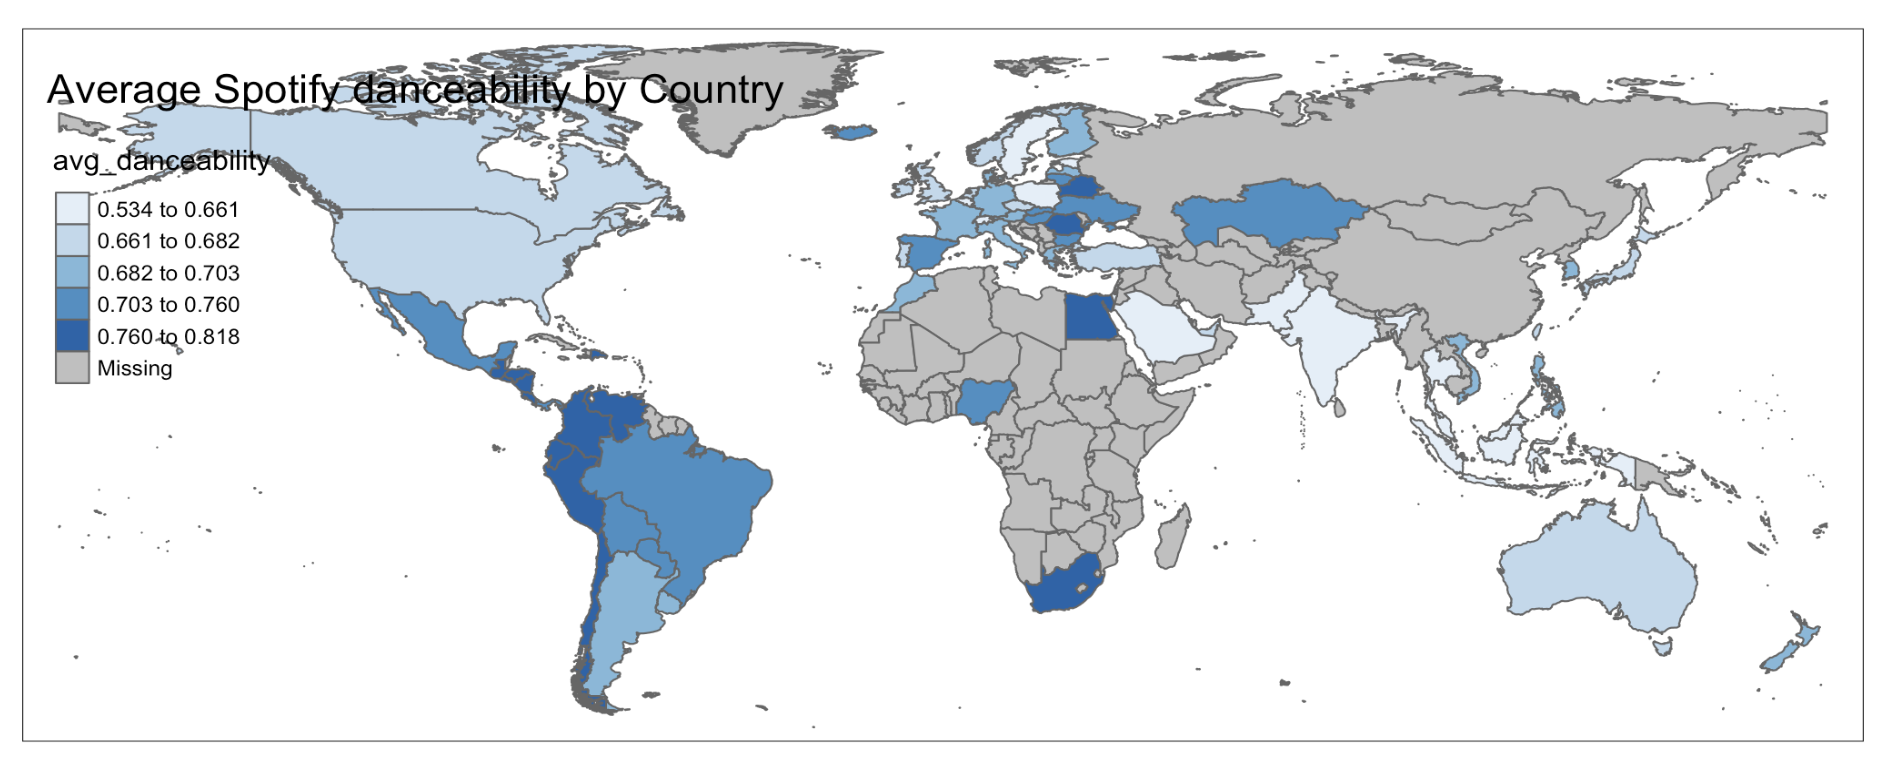
\includegraphics[width=0.7\linewidth]{Images/7_Geospatial/4_data2024/data2024_danceability.png}
    \caption{Mitjana de danceability de les noves dades}
    \label{fig:geo_mean_danceability}
\end{figure}

Primer de tot, observarem les mitjanes de cada país de diferents variables numèriques, començant per \textit{danceability}, a la figura \ref{fig:geo_mean_danceability}. Veiem que destaquen els països africans i també de Sud-amèrica, amb \textit{danceability} mitjana de més del 0.75\%. Això vol dir que aquestes zones tenen una gran diversitat en els estils musicals populars que són molt ballables. Tot i això, per exemple a Àfrica, continuen havent-hi bastants països amb NA així que tampoc podem generalitzar tant. El que és sorprenent, és que als Estats Units hi ha una mitjana de \textit{danceability} bastant moderada, però més baixa que a altres països i això pot voler dir que els gèneres que s'escolten no són tan ballables. En el cas d'Amèrica Llatina, els que tenen més alts són Colòmbia i Argentina, i després el Brasil. Ens quadren aquells nivells de \textit{danceability}, ja que aquesta zona té una forta tradició de música ballable en aquestes cultures, incloent-hi gèneres com la salsa, la bachata, la samba i reggaeton.

\begin{figure}[H]
    \centering
    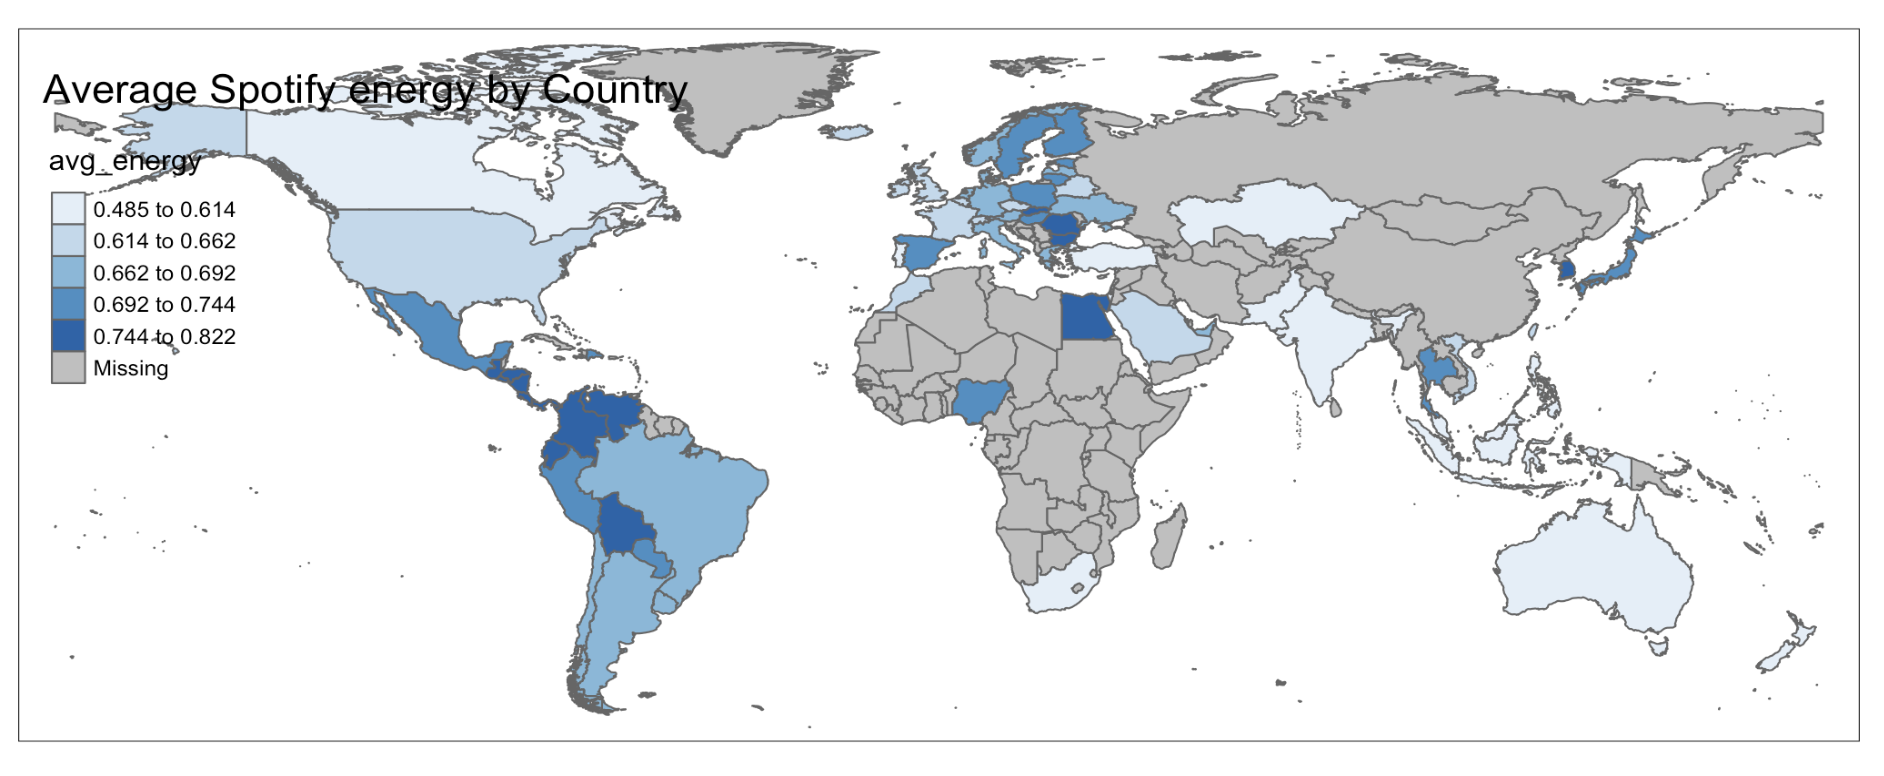
\includegraphics[width=0.7\linewidth]{Images/7_Geospatial/4_data2024/data2024_energy.png}
    \caption{Mitjana de Energy de les noves dades}
    \label{fig:geo_mean_energy}
\end{figure}

La variable Energy té una distribució molt semblant a la de danceability (\ref{fig:geo_mean_energy}), excepte alguns països, que són Sud-amèrica i Canadà. Veiem que els països a centre i Sud-amèrica fan cançons amb molta energia, amb vitalitat i un ritme vigorós. En el cas dels EUA té una energia moderada i el Canadà té una energia mitjana de les més baixes de totes. A Europa els nivells d'energia varien bastant, ja que a Espanya i els països nòrdics tenen música molt animada, pel fet que allà hi ha gèneres com dance i l'electrònica que són populars. En canvi, a França, o Regne Unit, tenen índexs més baixos, que podrien correspondre a estils musicals més suaus o melòdics com el Pop. Tenir aquesta visió global de l'energia de les cançons que s'escolten ens pot ajudar a entendre millor les preferències musicals regionals i pot ser útil per analistes, productors musicals i parques que busquen connectar amb audiències a través de la música a diferents parts del món.

\begin{figure}[H]
    \centering
    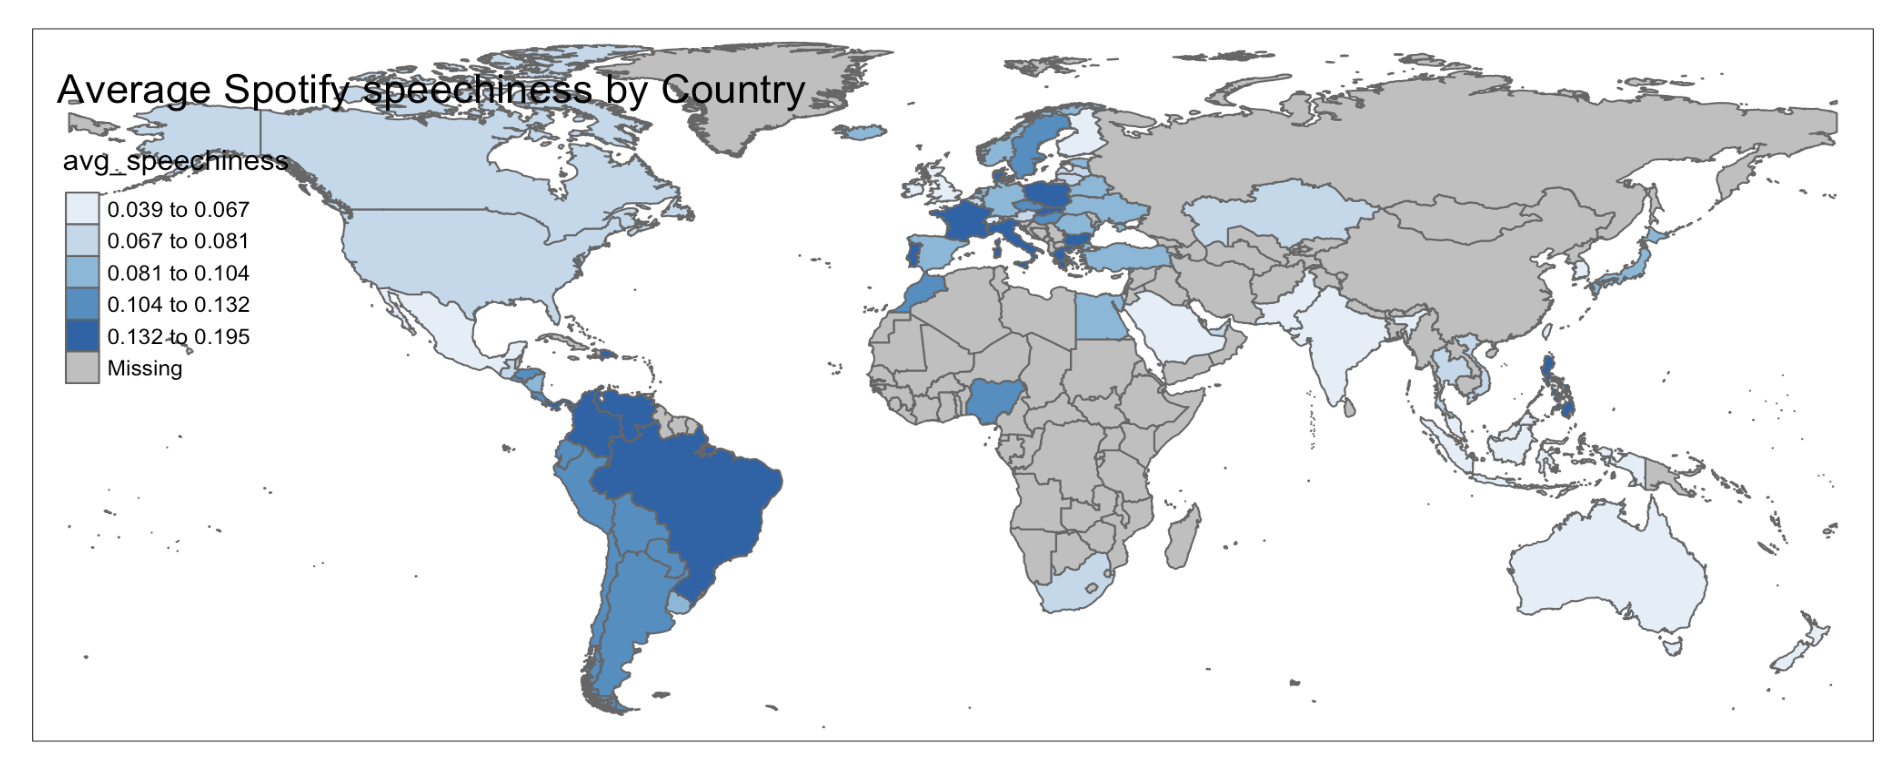
\includegraphics[width=0.7\linewidth]{Images/7_Geospatial/4_data2024/data2024_speechiness.png}
    \caption{Mitjana de Speechiness de les noves dades}
    \label{fig:geo_mean_speechiness}
\end{figure}

A continuació veiem la variable Speechiness \ref{fig:geo_mean_speechiness}. Aquí trobem una distribució diferent, ja que el país amb una mitjana més alta és el Brasil, seguit de Portugal, França. A Amèrica del Nord, mostren un nivell moderat a alt, el que pot reflectir que hi ha la presència de gèneres com el Hip-Hop o el rap. Veiem que els gèneres que s'escolten a Centreamèrica i Sud-amèrica (salsa o bachata) tenen menys speechiness. A Europa trobem una variabilitat considerable. Això es pot deure al fet que els diferents països escolten tipus de música diferents, i en el cas de França per exemple serà el Rap. Aleshores, aquesta variable ens pot ajudar a entendre millor la dinàmica de gèneres específics com el rap i el hip-hop en diferents cultures.

\begin{figure}[H]
\centering
    \begin{minipage}{.5\textwidth}
        \centering
        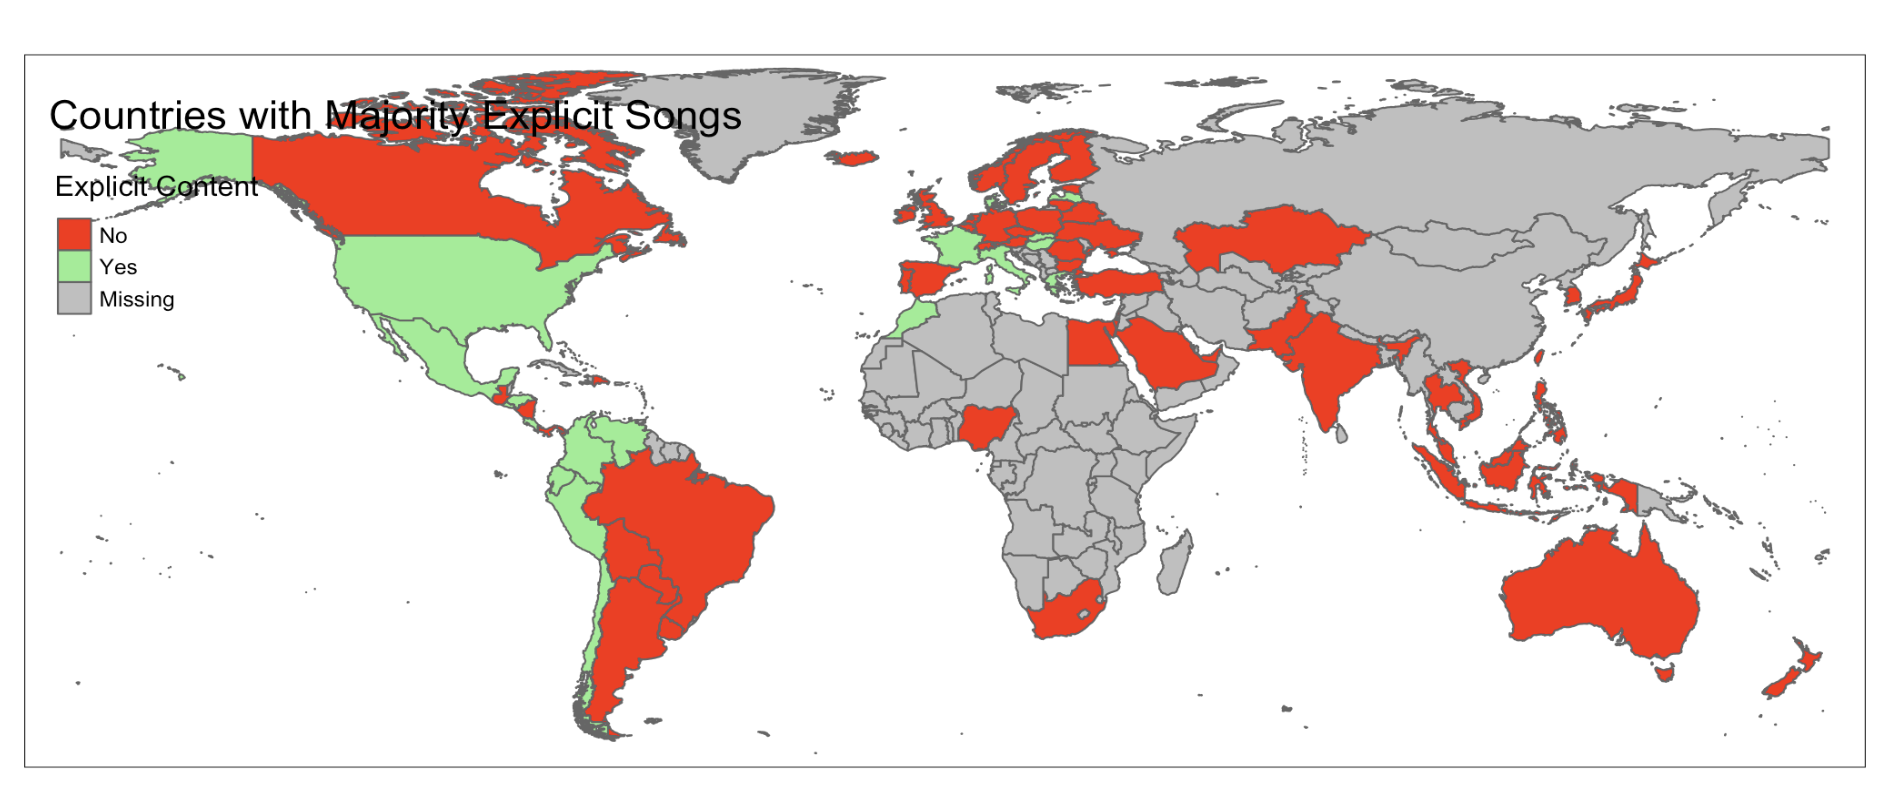
\includegraphics[width=0.99\linewidth]{Images/7_Geospatial/4_data2024/data2024_explicit_logic.png}
        \caption{Mapa de Explicit de les noves dades}
        \label{fig:geo_mean_explicit_logic}
    \end{minipage}%
    \begin{minipage}{.5\textwidth}
        \centering
        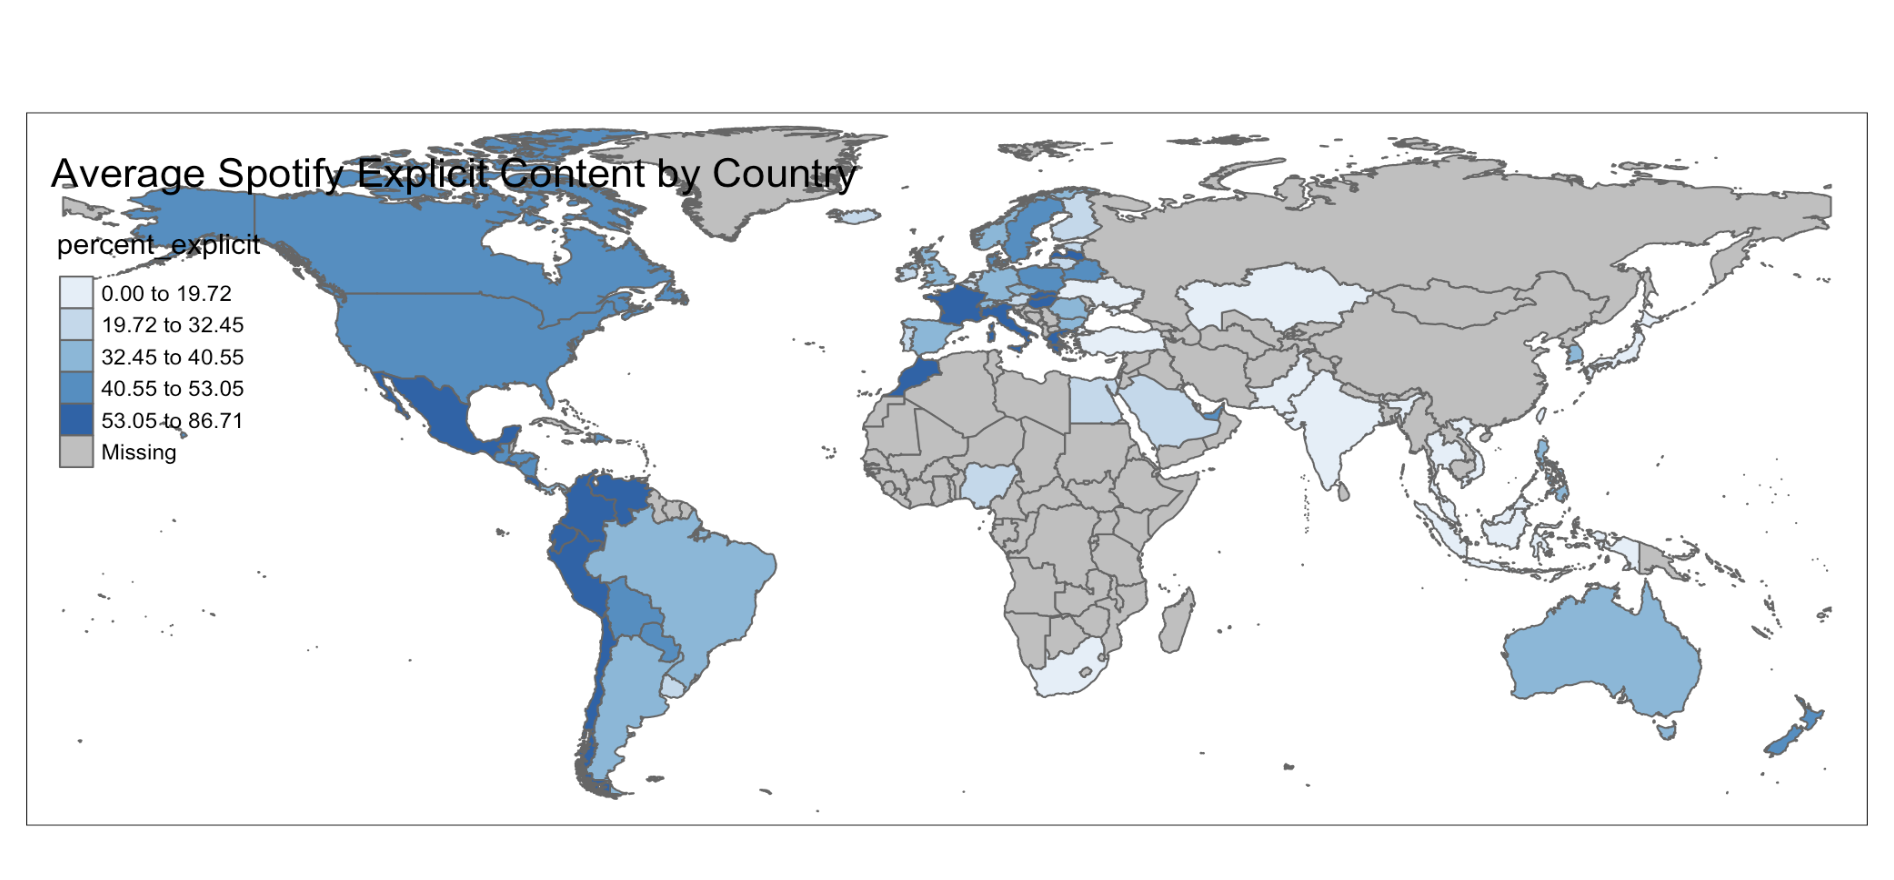
\includegraphics[width=0.99\linewidth]{Images/7_Geospatial/4_data2024/data2024_explicit.png}
        \caption{Mitjana de Explicit de les noves dades}
        \label{fig:geo_mean_explicit}
    \end{minipage}%
\end{figure}

Finalment, analitzen una de les úniques variables categòriques que hi ha a aquesta base de dades, explicit, a les figures \ref{fig:geo_mean_explicit_logic} i \ref{fig:geo_mean_explicit}. Volem saber quins països tendeixen a escoltar cançons explícites perquè ens ajudarà a entendre les diferències culturals i socials en el consum de la música. Veiem que la majoria dels països escolten més cançons no explícites que explícites, menys algunes excepcions. Aquest és el cas dels EUA, Mèxic, França, Itàlia i Centreamèrica. Això pot indicar una major acceptació o prevalença de llenguatge explícit en la música popular. També reflecteix diferències culturals dins de la regió quant a gustos o inclús normativa. El gènere que normalment inclouen cançons explícites és el hip-hop. A Àfrica i Àsia predominen les cançons no explícites.

\subsubsection{Conclusions}

Les conclusions del nostre anàlisi descriptiva geoespacial permeten identificar diverses aplicacions pràctiques i justificar la utilitat d'aquest estudi. Principalment, aquesta anàlisi ha revelat que la distribució d'artistes i les característiques de les seves cançons no són uniformes en l'àmbit global, sinó que mostren una tendència de concentració en àrees urbanes grans i centres culturals com els Estats Units i Europa. Això suggereix que aquestes zones, amb una alta concentració de recursos com estudis d'enregistrament i accessibilitat a professionals de la indústria musical, proporcionen millors oportunitats per al reconeixement en plataformes com Spotify.

En l'àmbit pràctic, els artistes emergents podrien beneficiar-se d'aquesta informació per orientar les seves estratègies de carrera. Per exemple, podrien considerar la possibilitat de traslladar-se o establir connexions professionals en aquests centres musicals per augmentar les seves oportunitats de ser descoberts o per desenvolupar col·laboracions més fructíferes.

Finalment, l'anàlisi geoespacial no només proporciona una fotografia de l'estat actual de la música en l'àmbit mundial, sinó que també ofereix informació sobre com les tendències musicals evolucionen amb el temps. Així, aquesta anàlisi es converteix en una eina valuosa per a la presa de decisions estratègiques en el context de la indústria musical global.

Addicionalment, ampliant la nostra informació amb dades sobre el consum (el top per països), hem pogut observar com existeixen també certes tendències en el tipus de cançó més popular en cada regió del món, en alguns casos observant fins i tot diferències importants en països veïns. 

\subsection{Anàlisi Geoespacial Tipus I: Geoestadística Clàssica (Variogrames i Kriging)}

La geoestadística clàssica es centra en l'anàlisi de dades espacials per modelar l'estructura de dependència espacial, d'aquesta manera entendrem com les nostres dades varien en l'espai, i posteriorment s'han realitzat interpolacions per predir valors en ubicacions no mostrejades. Principalment s'ha fet servir: \textbf{el variograma i kriging}.

\subsubsection{Selecció de la Variable: Energy}

En aquest anàlisi geoespacial, s'ha seleccionat la variable \textbf{energia} de les cançons per diversos motius. 

Cal destacar que l'energia és una característica important que pot influir en la percepció de la música i la seva popularitat. A més, la distribució de l'energia de les cançons pot reflectir patrons geogràfics interessants que poden estar relacionats amb preferències culturals o tendències musicals regionals.

Aquesta variable té una distribució aproximadament normal, lleugerament asimètrica cap a la dreta. Com es pot observar, la majoria de les cançons tenen valors d'energia entre 0.4 i 0.8.

\begin{figure}[h!]
    \centering
    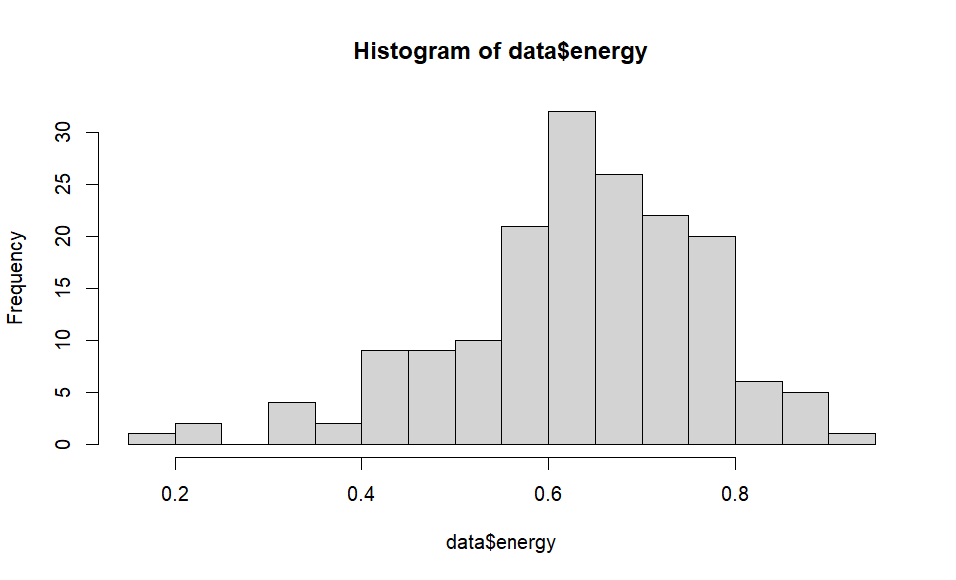
\includegraphics[width=0.85\linewidth]{histograma_energy.png}
    \caption{Histograma de la variable Energy}
    \label{fig:histogram_energy}
\end{figure}

\subsubsection{Variograma}

Primer de tot, s'ha realitzat un variograma que ens permet entendre la variabilitat espacial d'una variable, en aquest cas sobre la variable \textbf{energy}. El variograma ens mostra com varia aquesta variable en funció de la distància entre punts de mostreig.

Per a ajustar correctament el variograma a les nostres dades, vam seleccionar dos paràmetres clau: el cutoff i l'amplada (width).

\textbf{- Cutoff (10000 km):} Aquest paràmetre determina la distància màxima a la qual considerem les parelles de punts per al càlcul del variograma. Vam triar 10,000 km perquè la nostra base de dades inclou ciutats de tot el món. Això ens permet capturar la variabilitat espacial a llargues distàncies, la qual cosa és rellevant quan es treballa amb dades globals.

\textbf{- Width (500 km):} L'amplada defineix la mida dels intervals de distància en els quals agrupem les parelles de punts per calcular la semivariança. Vam triar 500 km per obtenir un bon equilibri entre la resolució espacial i el nombre de parelles de punts dins de cada interval. Això ens assegura que cada punt del variograma es basa en un nombre suficient de parelles de punts per ser estadísticament fiable.

\begin{figure}
    \centering
    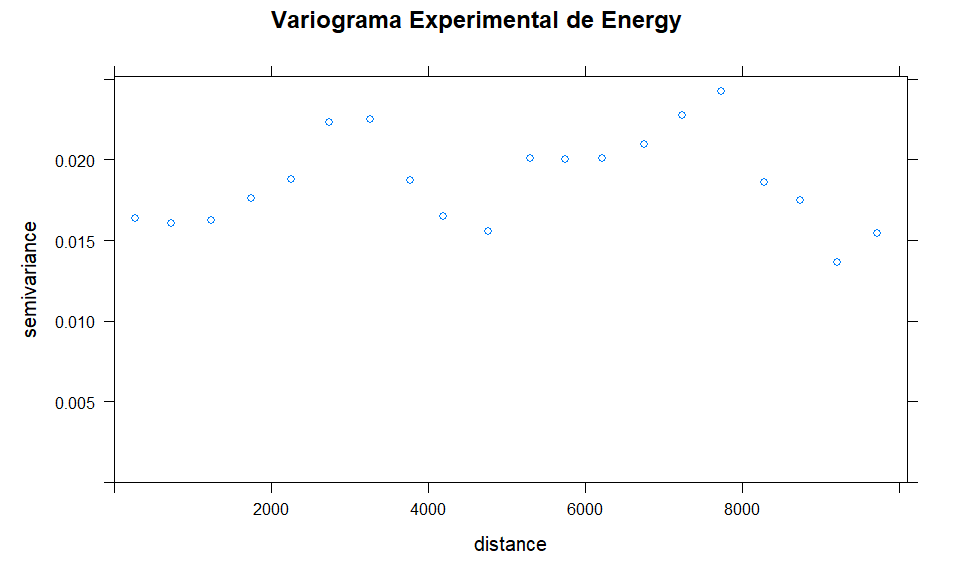
\includegraphics[width=0.75\linewidth]{variograma_experimental_energy.png}
    \caption{Variograma Experimental d'Energy}
    \label{fig:variograma_experimental_energy}
\end{figure}

Es pot observar que la semivariança comença en valors baixos per a distàncies curtes i augmenta fins a arribar a un pic al voltant de 2000-4000 km. Tot i que el variograma sembla tenir una tendència inicial a augmentar la semivariança amb l'augment de la distància entre punts, es pot observar que la variable \textbf{energy} no segueix un patró segons la distància. A mesura que augmenta la distància, la semivariança torna a augmentar i disminuir, mostrant una variabilitat significativa. 

Un cop triats els paràmetres, es va procedir a ajustar diversos models de variograma, per veure quin s'ajustava millor a les nostres dades. S'han considerat 3 models diferents per aquesta variable: esfèric, exponencial i gaussià.

Després d'ajustar-los, vam comparar-los per determinar quin s'ajustava millor a les nostres dades.

\begin{figure}[ht]
    \centering
    \begin{subfigure}[b]{0.32\textwidth}
        \centering
        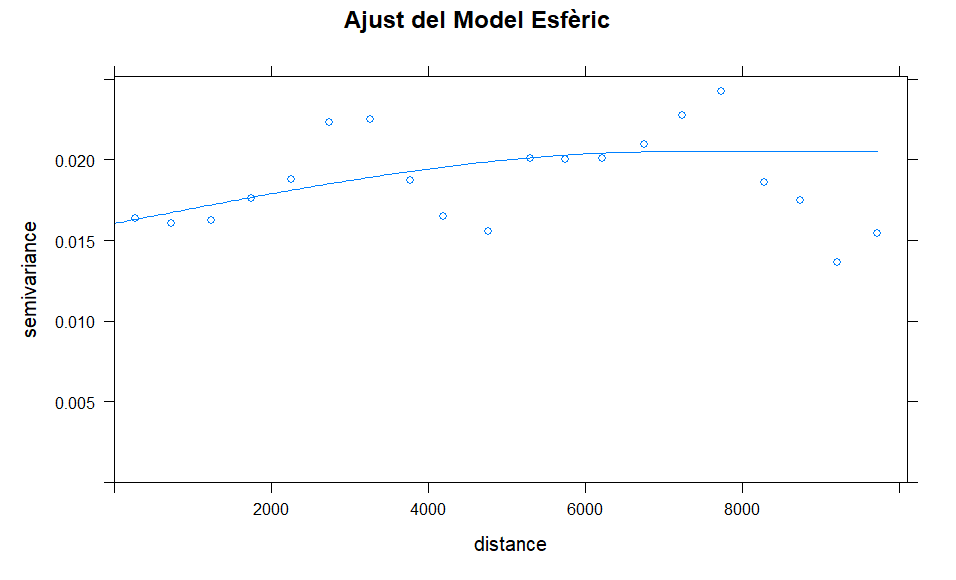
\includegraphics[width=\textwidth]{Images/7_Geospatial/2_modeling/model_esferic.png}
        \caption{Model Esfèric}
        \label{fig:esferic}
    \end{subfigure}
    \hfill
    \begin{subfigure}[b]{0.32\textwidth}
        \centering
        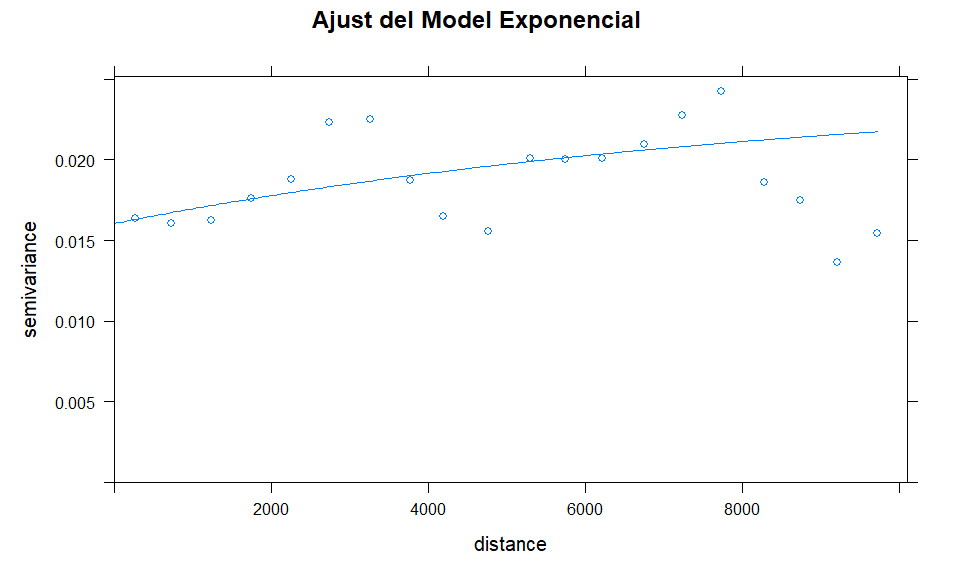
\includegraphics[width=\textwidth]{Images/7_Geospatial/2_modeling/model_exponencial.png}
        \caption{Model Exponencial}
        \label{fig:exponencial}
    \end{subfigure}
    \hfill
    \begin{subfigure}[b]{0.32\textwidth}
        \centering
        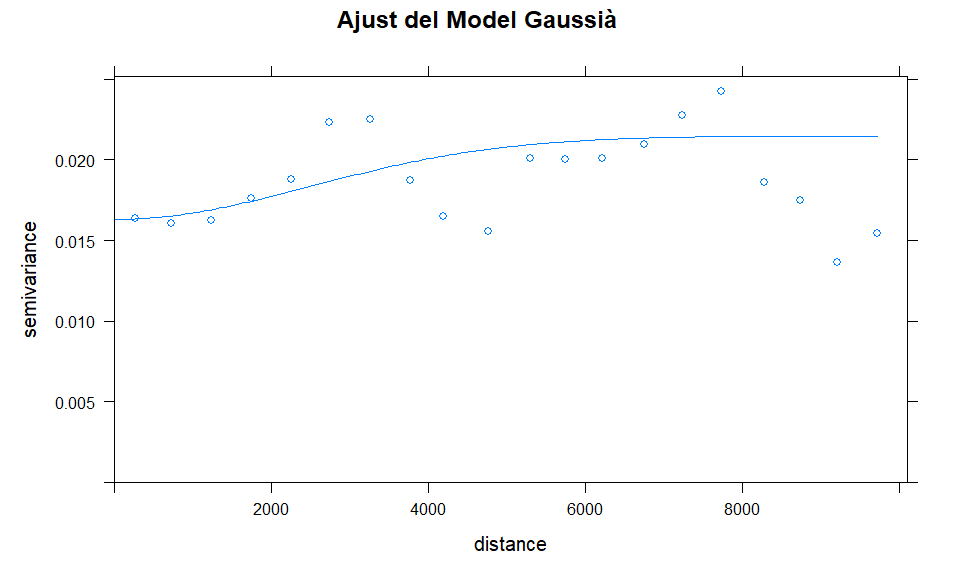
\includegraphics[width=\textwidth]{Images/7_Geospatial/2_modeling/model_gaussia.png}
        \caption{Model Gaussià}
        \label{fig:gaussian}
    \end{subfigure}
    \caption{Ajust dels diferents models de variograma per a la variable \textbf{energy}.}
    \label{fig:variograma_models}
\end{figure}

Aquesta comparació visual ens permet veure quin model segueix millor la tendència del variograma experimental. Triant el model més adequat, podem assegurar-nos que les interpolacions futures seran les més precises possibles. En aquest cas, vam optar pel model esferic, ja que s'ajustava millor a les nostres dades segons la visualització dels gràfics.

\subsubsection{Validació del Model}
Després de realitzar el variograma i ajustar els models, es va procedir a la validació del model per assegurar-nos que el model del variograma seleccionat s'ajusta adequadament a les dades. D'aquesta manera es pot avaluar la precisió i fiabilitat del model ajustat.

Per validar el model, s'ha utilitzat la tècnica de validació creuada amb el mètode Leave-One-Out Cross-Validation (LOOCV). D'aquesta manera es pot avaluar el rendiment del model en una situació de predicció realista.

Després de realitzar la validació creuada, els resultats obtinguts sobre les mètriques de rendiment del model són els següents: \\ \\

\textbf{- Error mitjà (ME):} 0.0002191755

L'error mitjà és molt proper a zero, el que indica que, de mitjana, les prediccions del model no tenen un desplaçament sistemàtic respecte als valors observats. Això vol dir que el model no té un biaix significatiu en les seves prediccions i que les desviacions positives i negatives s'equilibren.

\textbf{- Arrel de l'error quadràtic mitjà (RMSE):} 0.131647

L'RMSE és relativament baix, la qual cosa indica que els errors de predicció del model són petits, i per tant, les prediccions del model són generalment molt properes als valors observats.

\textbf{- Error quadràtic mitjà dels z-scores(MSRE):} 1.00725

L'MSRE molt proper a 1 ens indica que la variància del model està ben ajustada. La distribució dels errors normalitzats és consistent amb les expectatives teòriques del model de variograma ajustat.

Els resultats de les mètriques de validació suggereixen que el model de variograma ajustat és adequat per a les nostres dades. Per tant, ja es pot procedir amb la interpolació kriging per predir els valors de la variable \textbf{energy} en ubicacions no mostrejades amb la certesa de que les prediccions seran fiables.

\subsubsection{Interpolació amb Kriging}
Després d'ajustar el model de variograma, s'ha procedit a la interpolació mitjançant la tècnica de kriging. Aquesta tècnica permet predir valors en ubicacions no mostrejades, basant-se en el model de variograma ajustat.

S'ha utilitzat la interpolació kriging ordinària (Ordinary Kriging), que assumeix que la mitjana de la variable és desconeguda però constant. 

Per realitzar la interpolació, primer s'ha creat una quadrícula global que cobreix tot el món. Es va assegurar que només es consideressin punts que es troben sobre terra, filtrant aquells que cauen en l'oceà o en àrees no rellevants per a l'anàlisi.

Els resultats de la interpolació kriging es mostren en un mapa global, on es poden observar les prediccions de la variable \textbf{energy} en diferents regions del món.

\begin{figure}[h!]
    \centering
    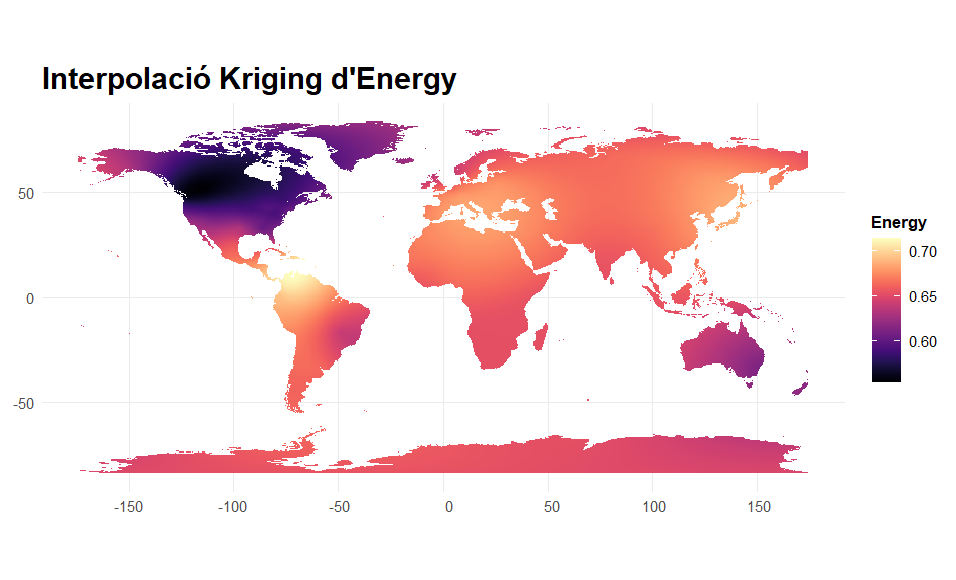
\includegraphics[width=0.95\linewidth]{interpolacio_energy.png}
    \caption{Interpolació Kriging d'Energy}
    \label{fig:interpolacio_energy}
\end{figure}

Com es pot observar a la figura anterior, les zones amb colors més càlids (groc i taronja) indiquen valors més alts d'energia, mentre que els colors més freds (lila i negre) indiquen valors més baixos.

\subsubsection{Conclusions}

Les observacions realitzades ens permeten extreure diverses conclusions importants sobre la distribució de l'energia de les cançons a nivell mundial, tal com es mostra a la figura de la interpolació Kriging.

\textbf{Zones amb major energia:}

- Amèrica del Sud i Central:
Les regions al top d'Amèrica del Sud, com Colòmbia, Equador i Veneçuela, així com parts d'Amèrica Central, mostren valors alts d'energia. Això pot estar relacionat amb la presència de gèneres musicals enèrgics com el reggaeton i la salsa, que són molt populars en aquesta zona.

- Zona del Mediterrani: 
Els països al voltant del Mar Mediterrani, incloent-hi parts d'Europa del Sud i del Nord d'Àfrica, també mostren valors alts d'energia.

- Rússia:
Les regions russes mostren una concentració d'energia elevada. Aquesta observació pot estar influenciada per la popularitat de la música pop i dance a Rússia.

- Japó: Al Japó, es detecten alts nivells d'energia, possiblement a causa de la influència del K-pop i altres gèneres musicals enèrgics que són molt populars en aquesta regió.

\textbf{Zones amb menor energia:}

- Canadà i part dels Estats Units: Les regions del Canadà i part dels Estats Units mostren valors més baixos d'energia. Això podria estar relacionat amb la preferència per gèneres musicals més tranquils i acústics en aquestes regions.

- Austràlia: A Austràlia, es troben valors baixos d'energia. Aquesta observació podria estar influenciada per una combinació de factors culturals i industrials dins de la indústria musical australiana.


Les observacions mostren una clara diversitat cultural i musical degut als diferents nivells d'energia en les cançons de cada zona. Els nivells d'energia en certes zones indiquen que les preferències culturals i les tradicions musicals tenen influència en els patrons d'energia que segueix cada regió. Aquesta informació pot ser útil per a la indústria musical per comprendre millor les preferències regionals i orientar les estratègies de màrqueting.

\subsection{Anàlisi Geoespacial Tipus I: Dades de reproduccions per països}
En l'apartat anterior, s'ha pogut analitzar i modelar les dades en funció del lloc de naixement dels artistes. D'aquesta manera, podiem saber de forma aproximada quin tipus de música es creen els artistes més populars globalment a cada regió del món, però amb les dades de les que disposàvem no podiem obtenir la informació sobre els oients. Per aquest motiu, es va decidir utilitzar en aquest apartat una altra base de dades que conté la informació sobre el top 50 de Spotify en 73 països diferents cada dia \cite{asaniczka2024top}.


Per aquest apartat, aquesta base de dades s'ha processat per tal d'obtenir informació útil pel modelatge geoespacial. Aquest ha consistit en agrupar totes les dades, utilitzant mitjanes i modes, en tan sols 73 punts (és a dir, la mitjana dels valors per país, i la mitjana de tots els dies). D'aquesta manera, s'ha buscat aconseguir una base de dades que expliqui (encara que sigui de forma aproximada) les tendències en els tipus de música més escoltats en cada país. Evidentment, també s'ha realitzat el procés per obtenir les coordenades (de cada país en aquest cas). Es poden observar els punts a \ref{fig:geo_new_map}.

\begin{figure}[H]
    \centering
    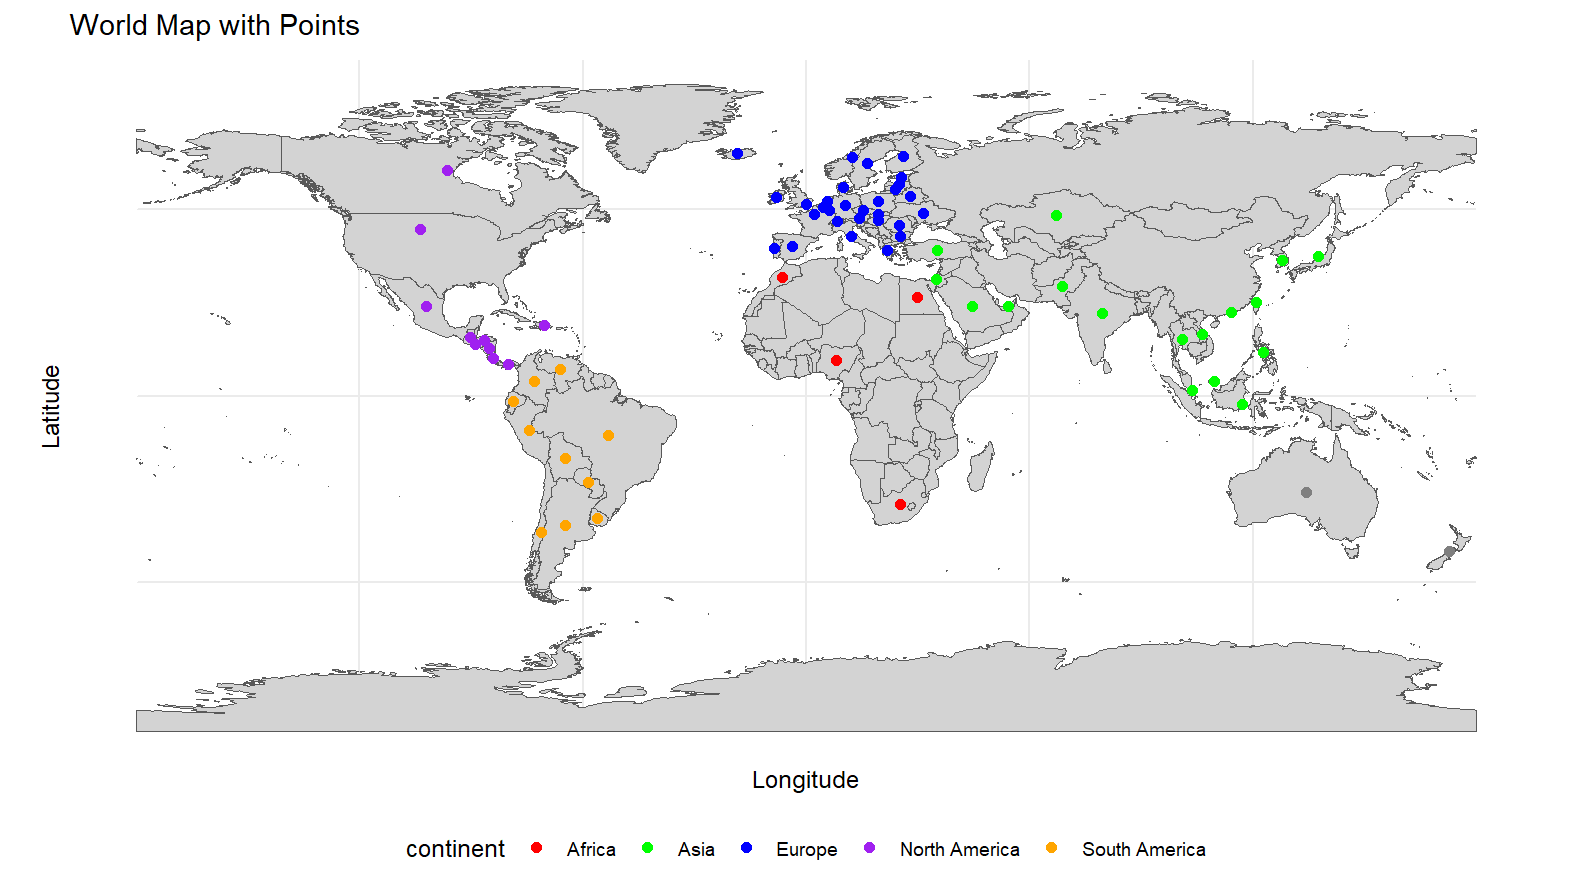
\includegraphics[width=0.5\linewidth]{Images//7_Geospatial//3_new/worldmap_points.png}
    \caption{Mapa de punts de les noves dades}
    \label{fig:geo_new_map}
\end{figure}

L'anàlisi s'ha realitzat per 3 variables diferents: la energia, per tal de poder comparar els resultats amb els obtinguts utilitzant els artistes; la popularitat de les cançons, per tal de determinar si els gustos musicals d'un país són més o menys regionals (ja que la popularitat es mesura a tot el món, per tant una popularitat més baixa en aquest cas indica que aquella cançó és popular tan sols en aquell país); i finalment la variable \textit{valence}, que indica la positivitat, per mirar de detectar tipus de música que s'escolten i relacionar-los amb la cultura del país.

Comentar que el procés d'obtenció dels variogrames i de la interpol·lació, al haver-se explicat en l'apartat anterior, es comentarà més per sobre en aquest, sense entrar tant en profunditat.

\subsubsection{Energy}

El primer pas per poder realitzar el modelatge és determinar uns valors de \textit{cutoff} i de \textit{width}. En la base de dades anterior, es van escollir els valors 10.000 i 500, ja que les dades de les que disposàvem estaven molt disperses. El variograma d'\textit{energy} utilitzant aquestes noves dades es pot apreciar a la figura \ref{fig:geo_new_energy_old}.

\begin{figure}[H]
    \centering
    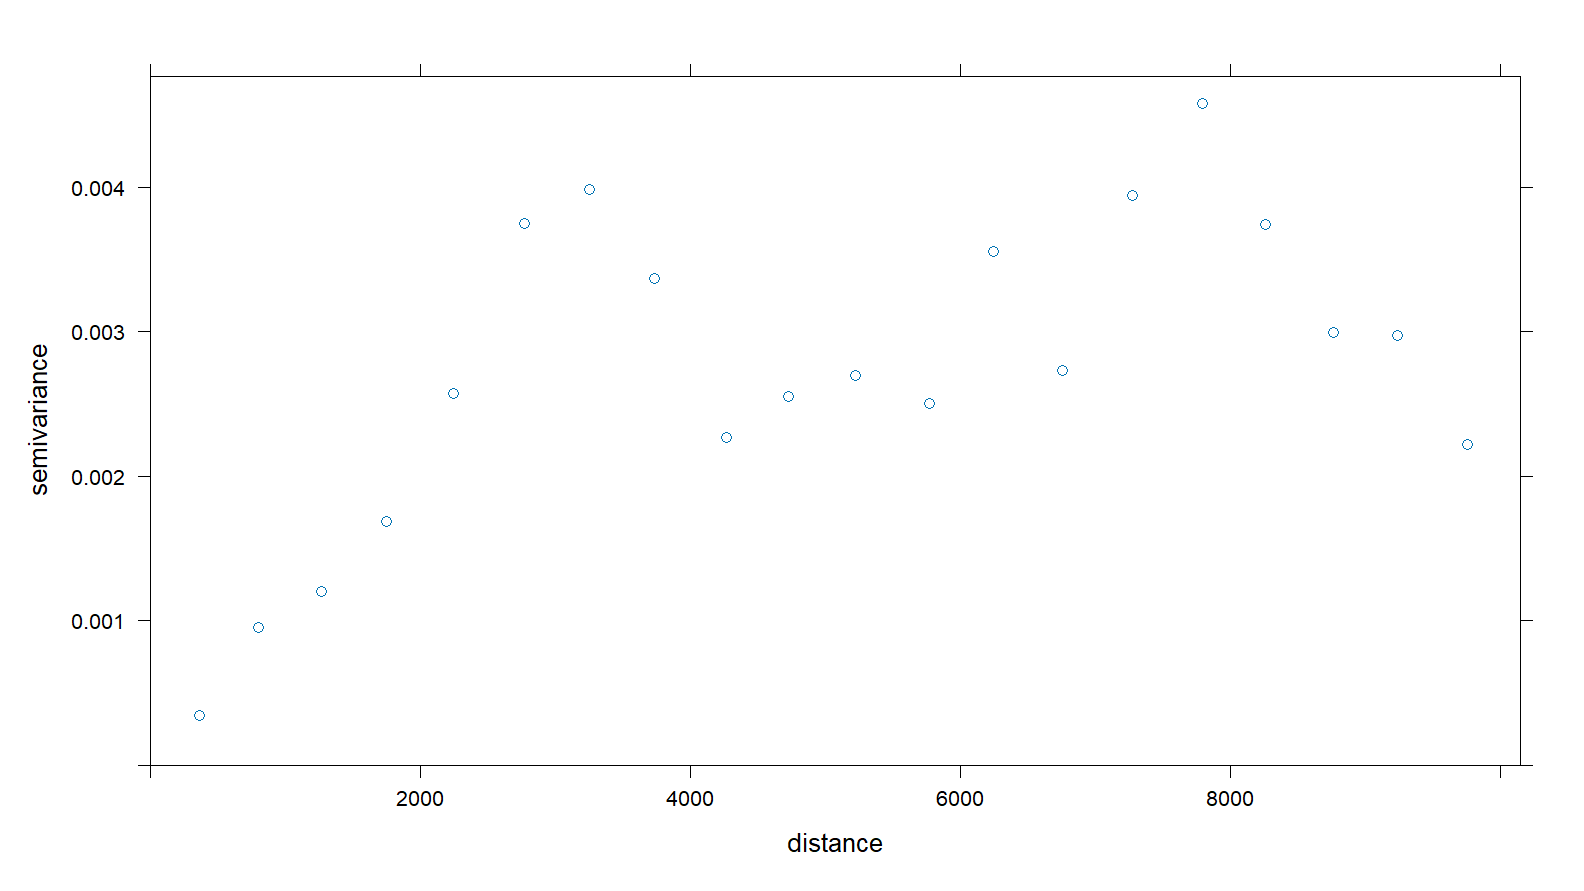
\includegraphics[width=0.75\linewidth]{Images//7_Geospatial//3_new/energy_10000_500_variogram.png}
    \caption{Variogram d'energy amb el mateix cutoff i width}
    \label{fig:geo_new_energy_old}
\end{figure}

Es va considerar que, per aquests nous punts, aquest variograma no tenia una forma prou adequada com per realitzar el modelatge. Com a alternativa, s'ha utiltizat un cutoff de 5000 i width de 300, quedant el variograma tal que \ref{fig:geo_new_energy}

\begin{figure}[H]
    \centering
    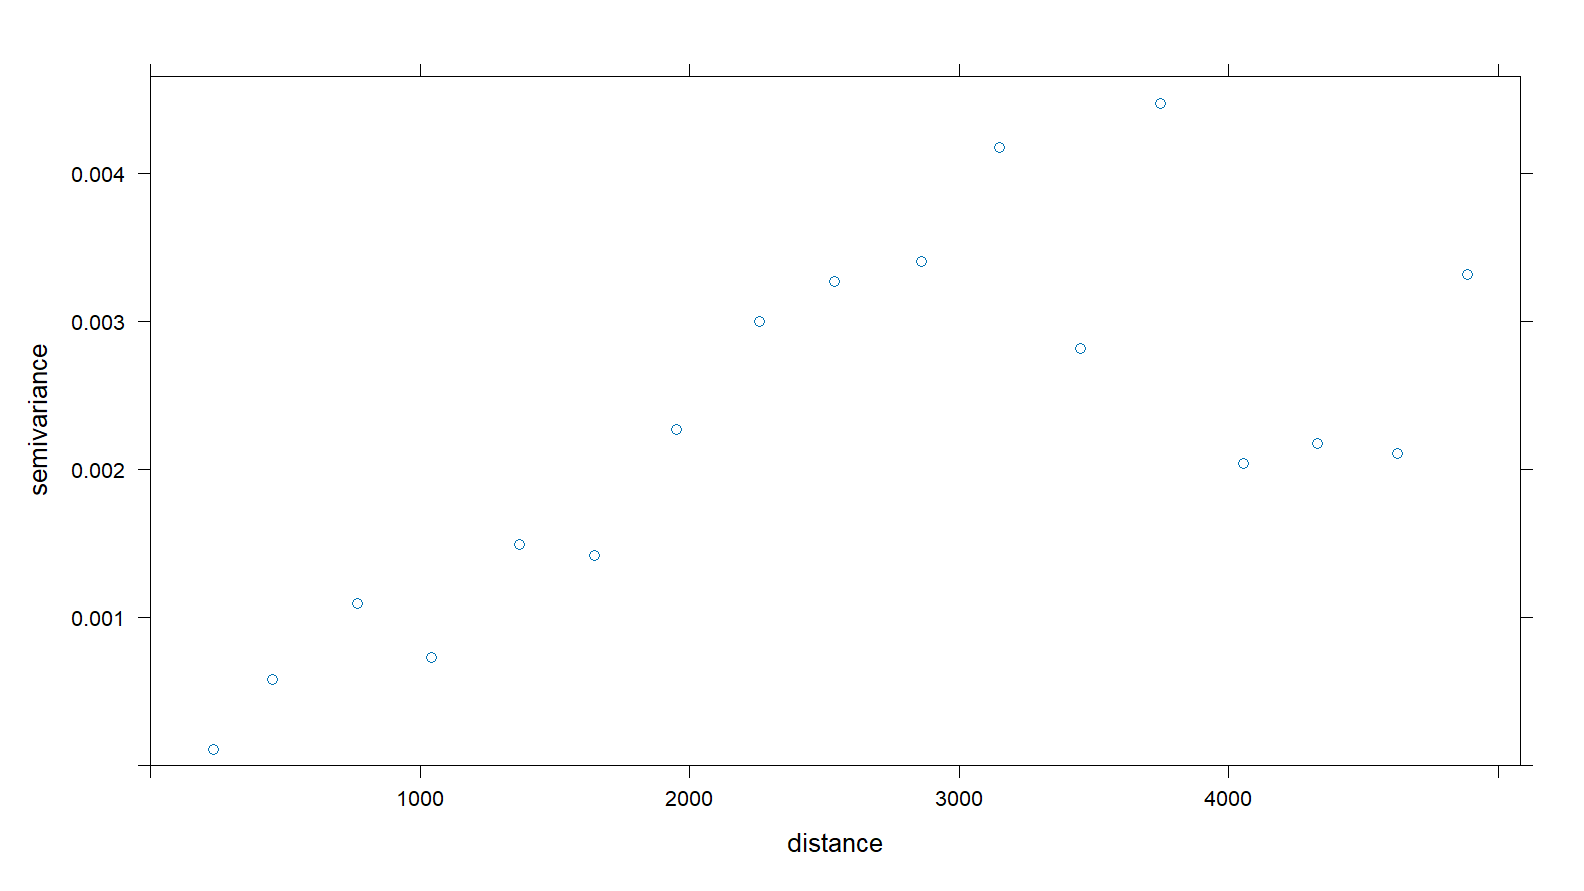
\includegraphics[width=0.75\linewidth]{Images//7_Geospatial//3_new/energy_5000_300_variogram.png}
    \caption{Variograma d'energy amb cutoff 5000 i width 300}
    \label{fig:geo_new_energy}
\end{figure}

Aquest, si bé té alguns punts que s'allunyen bastant de la resta, té un augment inicial que es podrà modelar. A veure que a continuació baixava una mica, es va optar per intentar utilitzar un model Wave. El seu psill és de 0.0025, amb un rang de 2200 i un nugget de 0.0002 (pràcticament parteix des de 0)\ref{fig:geo_new_energy_fit}.

\begin{figure}[H]
    \centering
    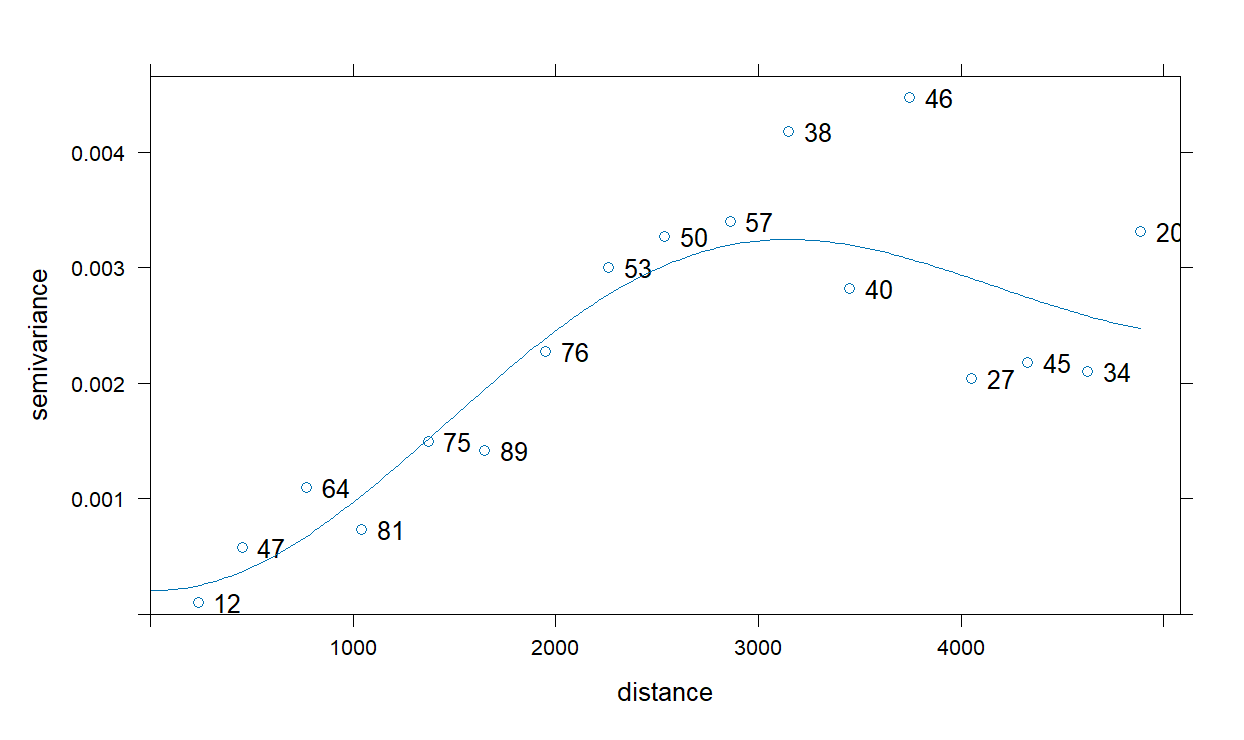
\includegraphics[width=0.5\linewidth]{Images//7_Geospatial//3_new/energy_variogram_fit.png}
    \caption{Fit del variograma Wave en energy}
    \label{fig:geo_new_energy_fit}
\end{figure}

Calculant les mètriques d'aquest model, vam observar un error mig de -0.0005 (bastant correcte), amb un RMSE de 0.049 i un MSRE de 3.57. Aquest últim valor és més elevat del que busquem idealment, ja que ens interessa que estigui entorn a 1, però tot i això, considerant el variograma, és prou bo.

Un cop obtingut aquest model, podem realitzar una interpol·lació pel grid de tot el món utilitzant kriging (ordinari altre cop. En aquest cas, es podria arribar a assumir que es coneix la mitjana si considerèssim les dades del top 50 global com a representatives de cada regió, però cal tenir en compte que diferents països tenen diferent nombre d'oients... i per tant no seria una assumpció vàlida). El resultat és la figura \ref{fig:geo_new_energy_interpol}.

\begin{figure}[H]
    \centering
    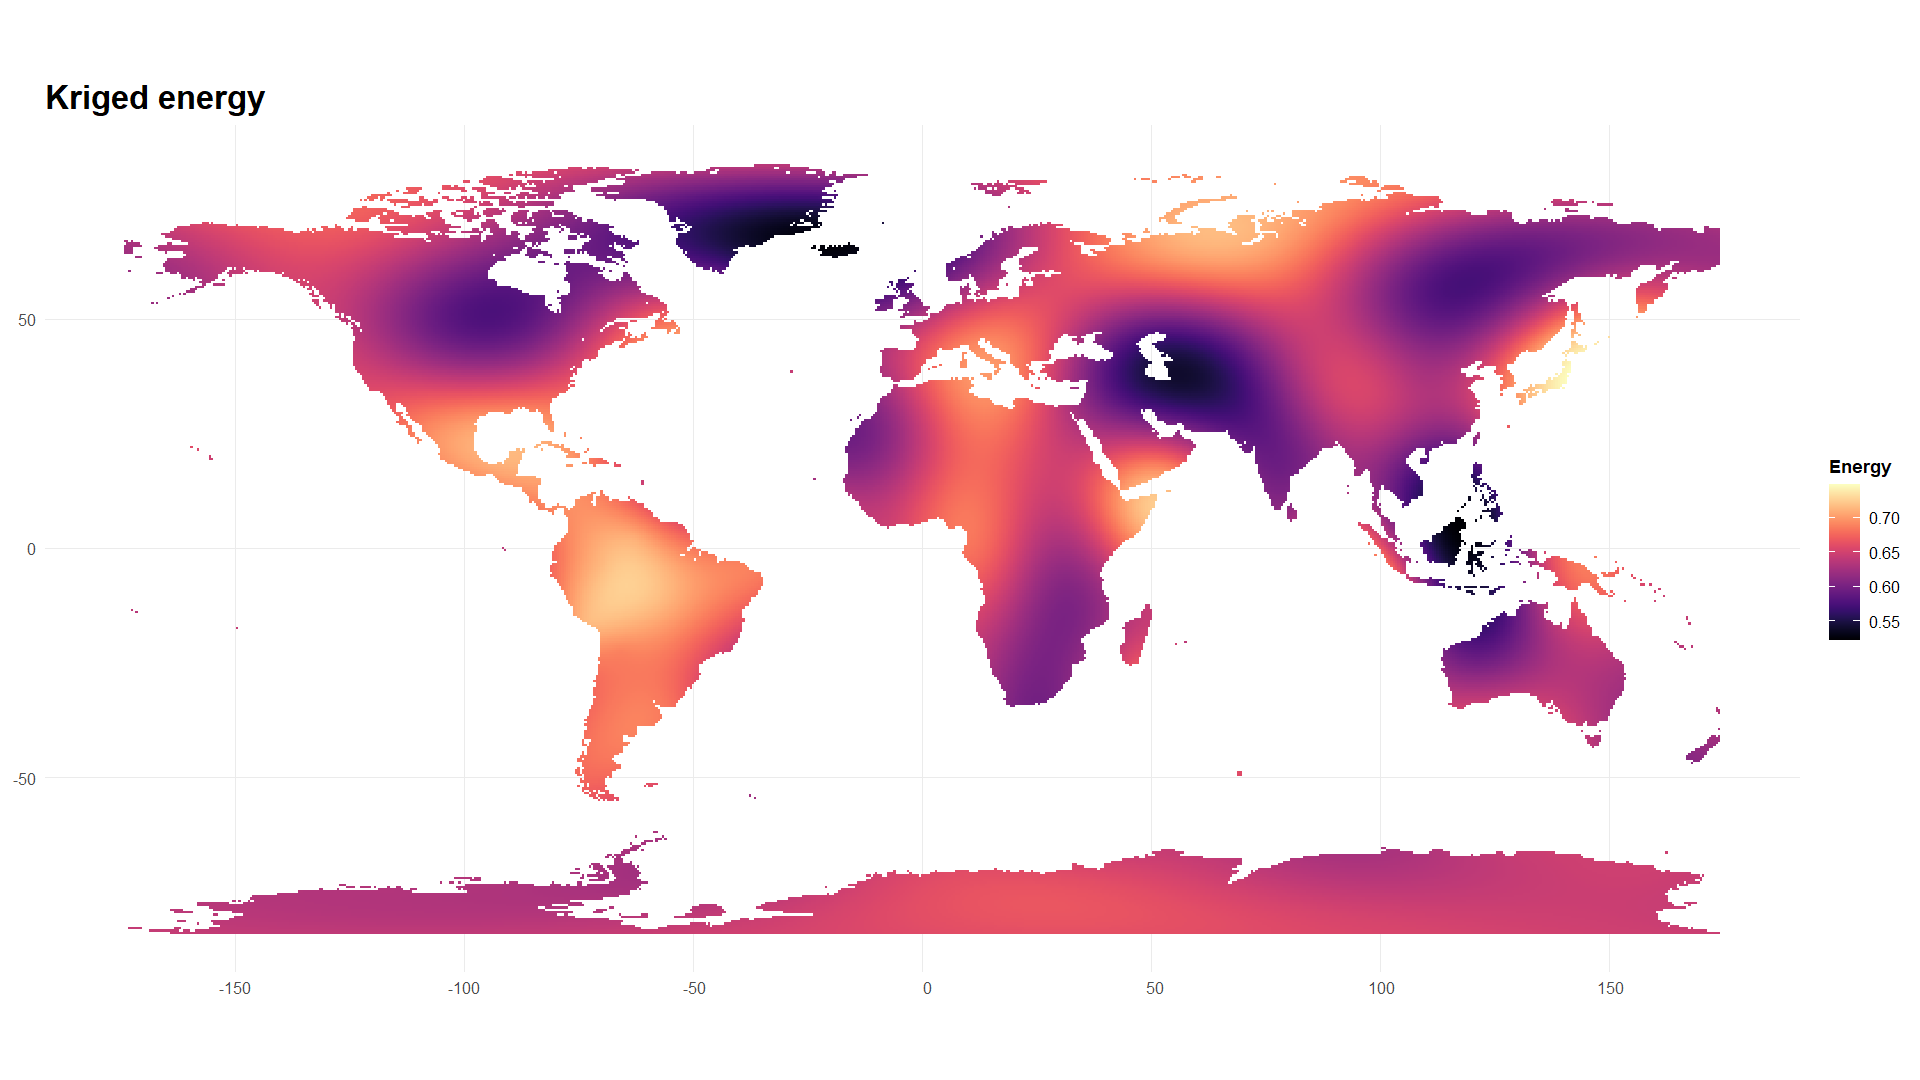
\includegraphics[width=0.8\linewidth]{Images//7_Geospatial//3_new/energy_interpolation.png}
    \caption{Interpol·lació usant kriging d'energy}
    \label{fig:geo_new_energy_interpol}
\end{figure}

Al observar el valor de MSRE del variograma, es va considerar que es podria obtenir un altre de millor. Després de realitzar certes proves, i canviant el cutoff a 4000 i el width a 400, es va obtenir un variograma que assolia un MSRE de 1.36 (molt més proper al valor òptim) \ref{fig:geo_new_energy_fit2}. Aquest és un model esfèric (Sph), amb psill 0.0035, 3500 de rang i 0.0001 de nugget (altre cop pràcticament 0, no tenim punts gaire propers). El resultat de la interpol·lació és observable a la figura \ref{fig:geo_new_energy_interpol2}.

\begin{figure}[H]
    \centering
    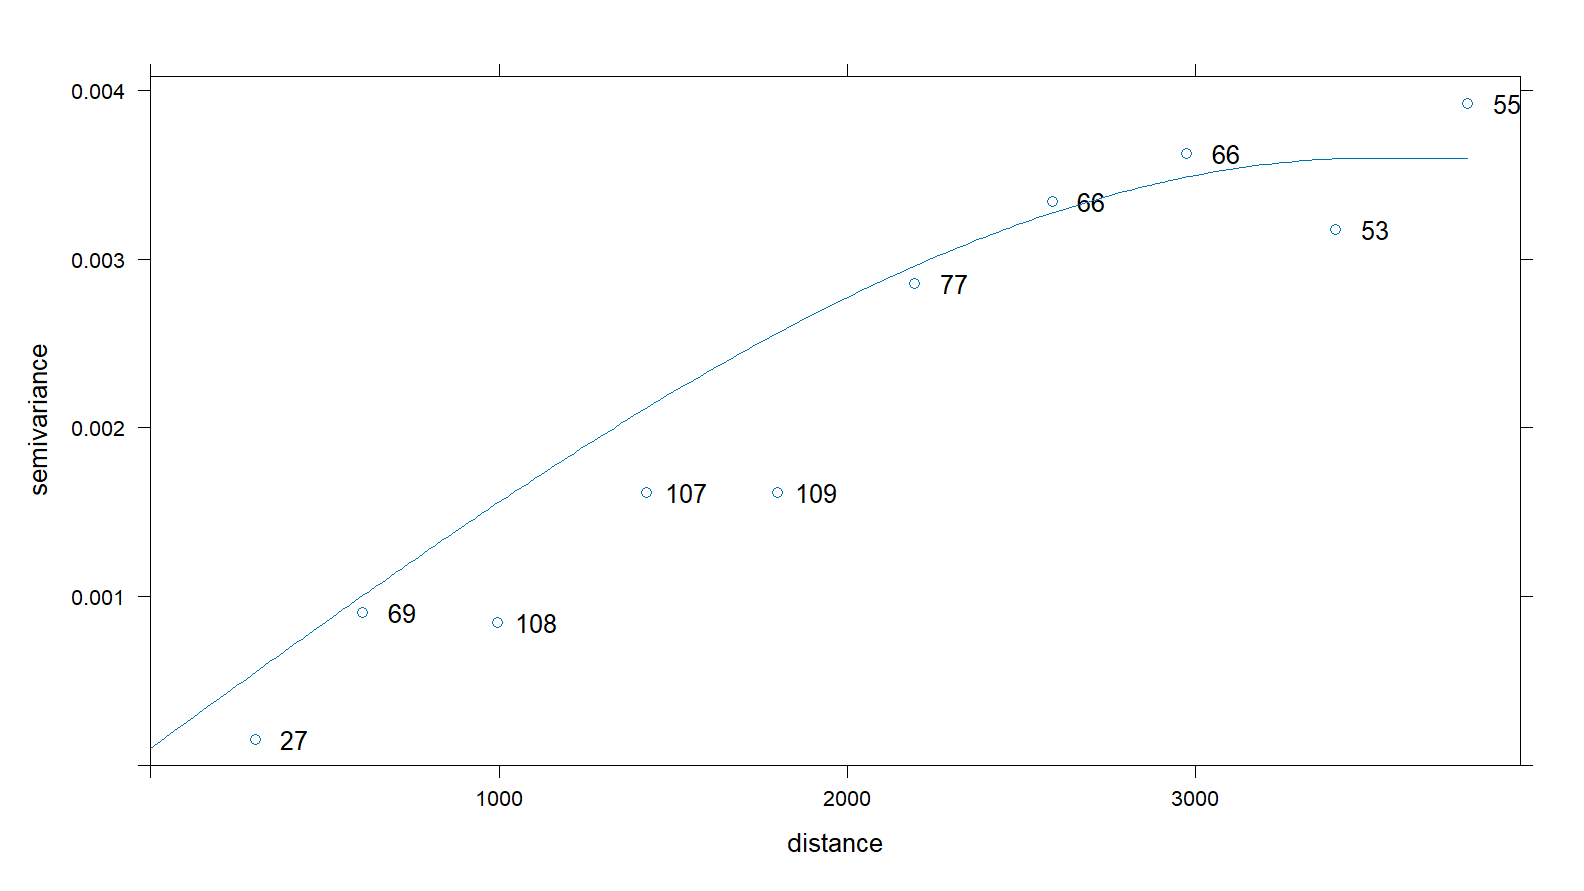
\includegraphics[width=0.5\linewidth]{Images//7_Geospatial//3_new/variograma_energy_new2.png}
    \caption{Fit del nou variograma en energy}
    \label{fig:geo_new_energy_fit2}
\end{figure}

\begin{figure}
    \centering
    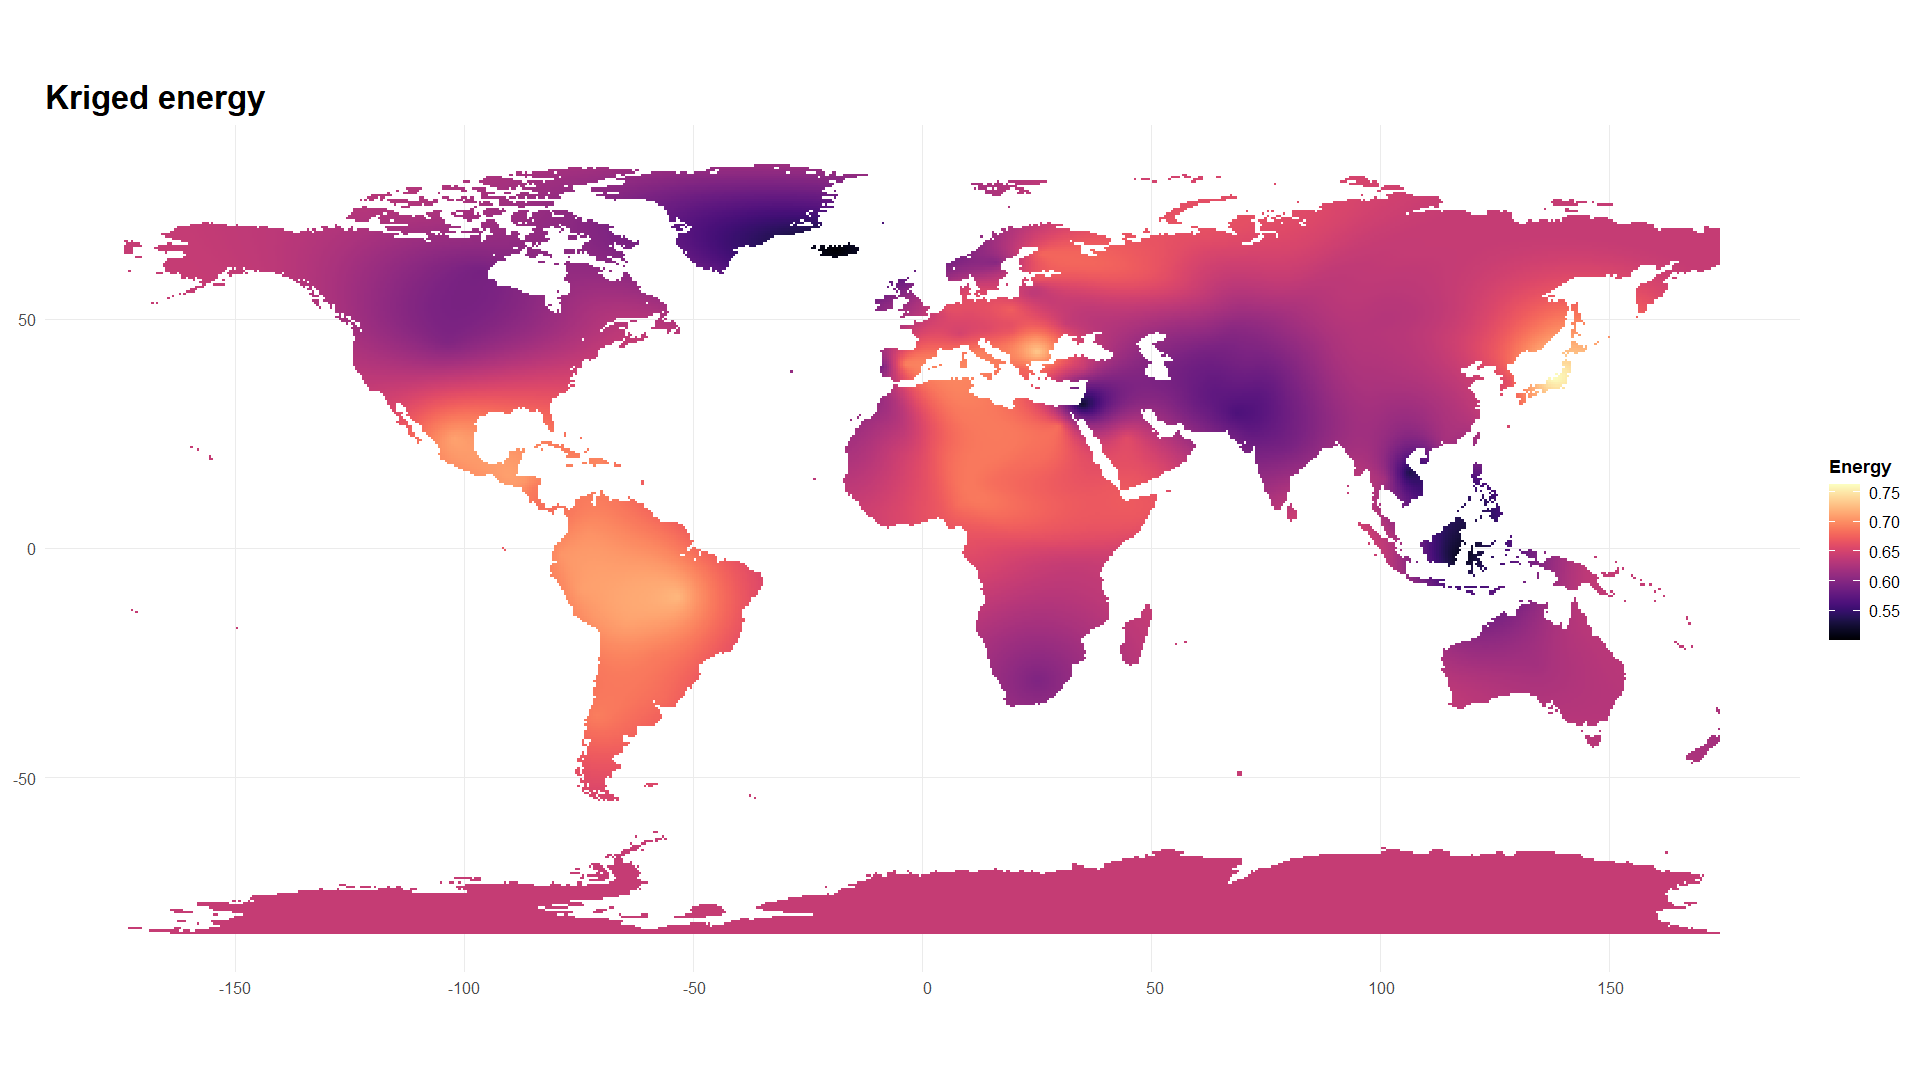
\includegraphics[width=0.8\linewidth]{Images//7_Geospatial//3_new/energy_interpolation_2.png}
    \caption{Interpol·lació usant el nou variograma d'energy}
    \label{fig:geo_new_energy_interpol2}
\end{figure}

Comparant els dos, s'observa com en aquest segon no hi ha una concentració elevada d'\textit{energy} al nord de Rússia, per exemple (punt llunyà d'on no tenim dades), ni hi ha una concentració tan baixa a la zona d'Orient mitjà. En general, és menys extrem.

Aquests resultats es poden contextualitzar amb els de l'apartat anterior \ref{fig:interpolacio_energy}, on observàvem la distribució d'energia segons els artistes. En general, sembla ser que els hàbits de consum de la gent d'una regió i la música que creen són bastant similars: seguim observant la zona d'Amèrica del Nord amb concentracions baixes d'energia, mentre que Amèrica del Sud, Japó i el Mediterrani destaquen per tenir concentracions elevades.

Observem algunes diferències a la zona de Tailàndia, Indonèsia i Filipines, així com Orient Pròxim, que en la interpol·lació per artistes tenien valors bastant més elevats que en l'actual. A més, en aquest cas Islàndia és el punt amb menys energia, enlloc dels Estats Units d'Amèrica. 

Aquestes diferències es deuen en part al fet que, per artistes, no disposàvem de dades d'aquests llocs (no apareixia cap artista del sud asiàtic, ni d'Àfrica. Tot i això, sembla ser que hi ha certa relació entre la energia de música que crea la gent d'un país i la de la música que escolten més els seus compatriotes.

\subsubsection{Track Popularity}

Utilitzar aquests dades per país també ens permet obtenir informació sobre com es compara aquella música amb la més escoltada globalment, utilitzant popularity. Aquesta és una mètrica assignada per Spotify en funció de les reproduccions que rep una cançó en tot el món. D'aquesta manera, es podrà saber si la música del top 50 d'un país és més "local", és a dir només s'escolta allà, o s'escolta a tot el món.

El variograma s'ha creat usant un cutoff de 6000 i width de 400. Observant-lo, s'ha considerat que un model esfèric es podria ajustar correctament a aquestes semivariàncies. Inicialment, es va usar un psill de 50, amb range de 2000 i nugget de 7, però després d'acabar de refinar aquest ajust utiltizant fit.variogram, els valors obtinguts són 65.4, 2262 i 1.76 respectivament. Les mètriques són bastant bones, ME de -0.098, MSRE de 1.048 i RMSE de 6.07 (més elevat que en \textit{energy}, però cal tenir en compte que aquests valors són entre 0 i 100 i energy entre 0 i 1).

\begin{figure}[H]
    \centering
    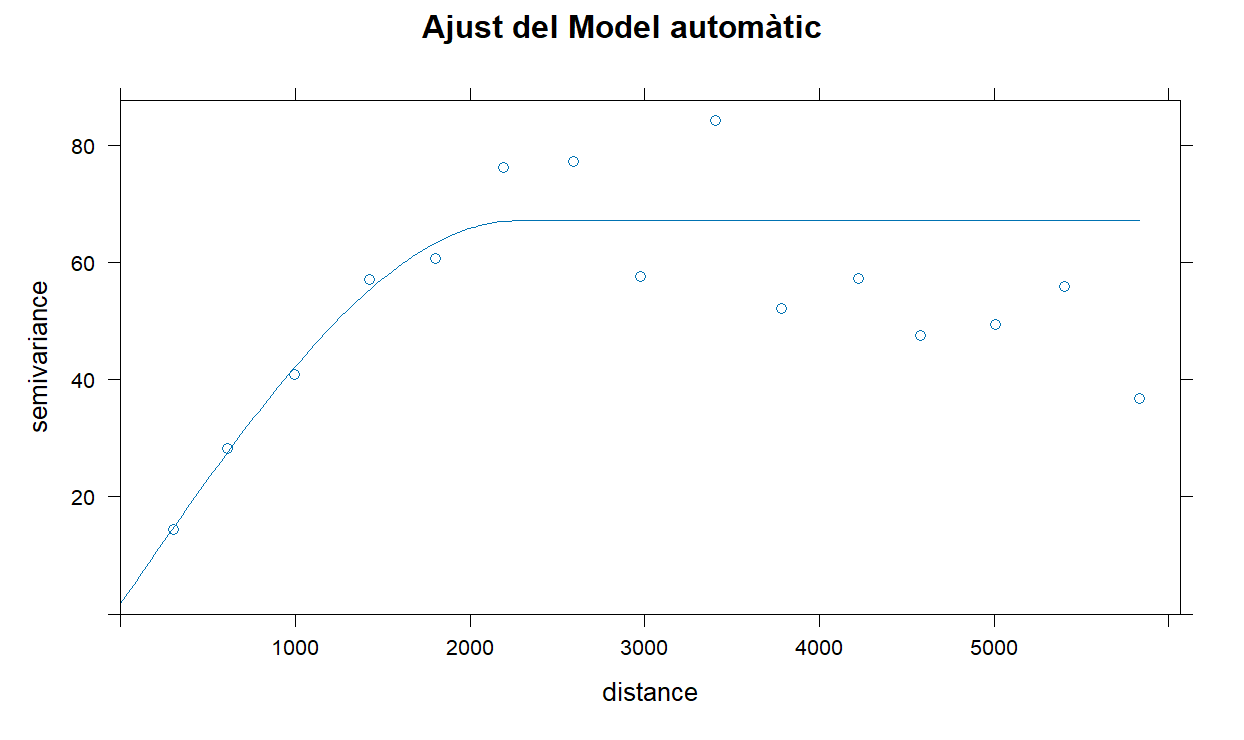
\includegraphics[width=0.5\linewidth]{Images//7_Geospatial//3_new/variogram_fit_popularity.png}
    \caption{Variograma ajustat (automàticament) per la popularitat}
    \label{fig:geo_new_pop_variogram}
\end{figure}

S'observa en \ref{fig:geo_new_pop_variogram} com s'ajusta prou bé a les dades, especialment als 5 primers punts. A partir d'allà, hi ha algunes distàncies amb valors estranys, però tot i axí es manté en un punt prou bo. La interpol·lació s'observa a la fiugra \ref{fig:geo_new_pop_interpol}

\begin{figure}[H]
    \centering
    
\includegraphics[width=0.8\linewidth]{Images//7_Geospatial//3_new/popularity_interpolation.png}
    \caption{Interpol·lació usant kriging de la popularitat}
    \label{fig:geo_new_pop_interpol}
\end{figure}

En aquest cas, tota Amèrica té valors molt elevats. Alhora, Austràlia i El regne unit també tenen valors molt elevats. Dastaca també, de forma sorprenent, la zona dels Emirats Àrabs Units (Dubai...). Les zones amb valors més negatius, és a dir, música més regional, són l'est d'Europa (sobretot Grècia, tot i que també més cap al nord), així com Egipte, el Marroc, o Islàndia.

\begin{figure}[H]
    \centering
    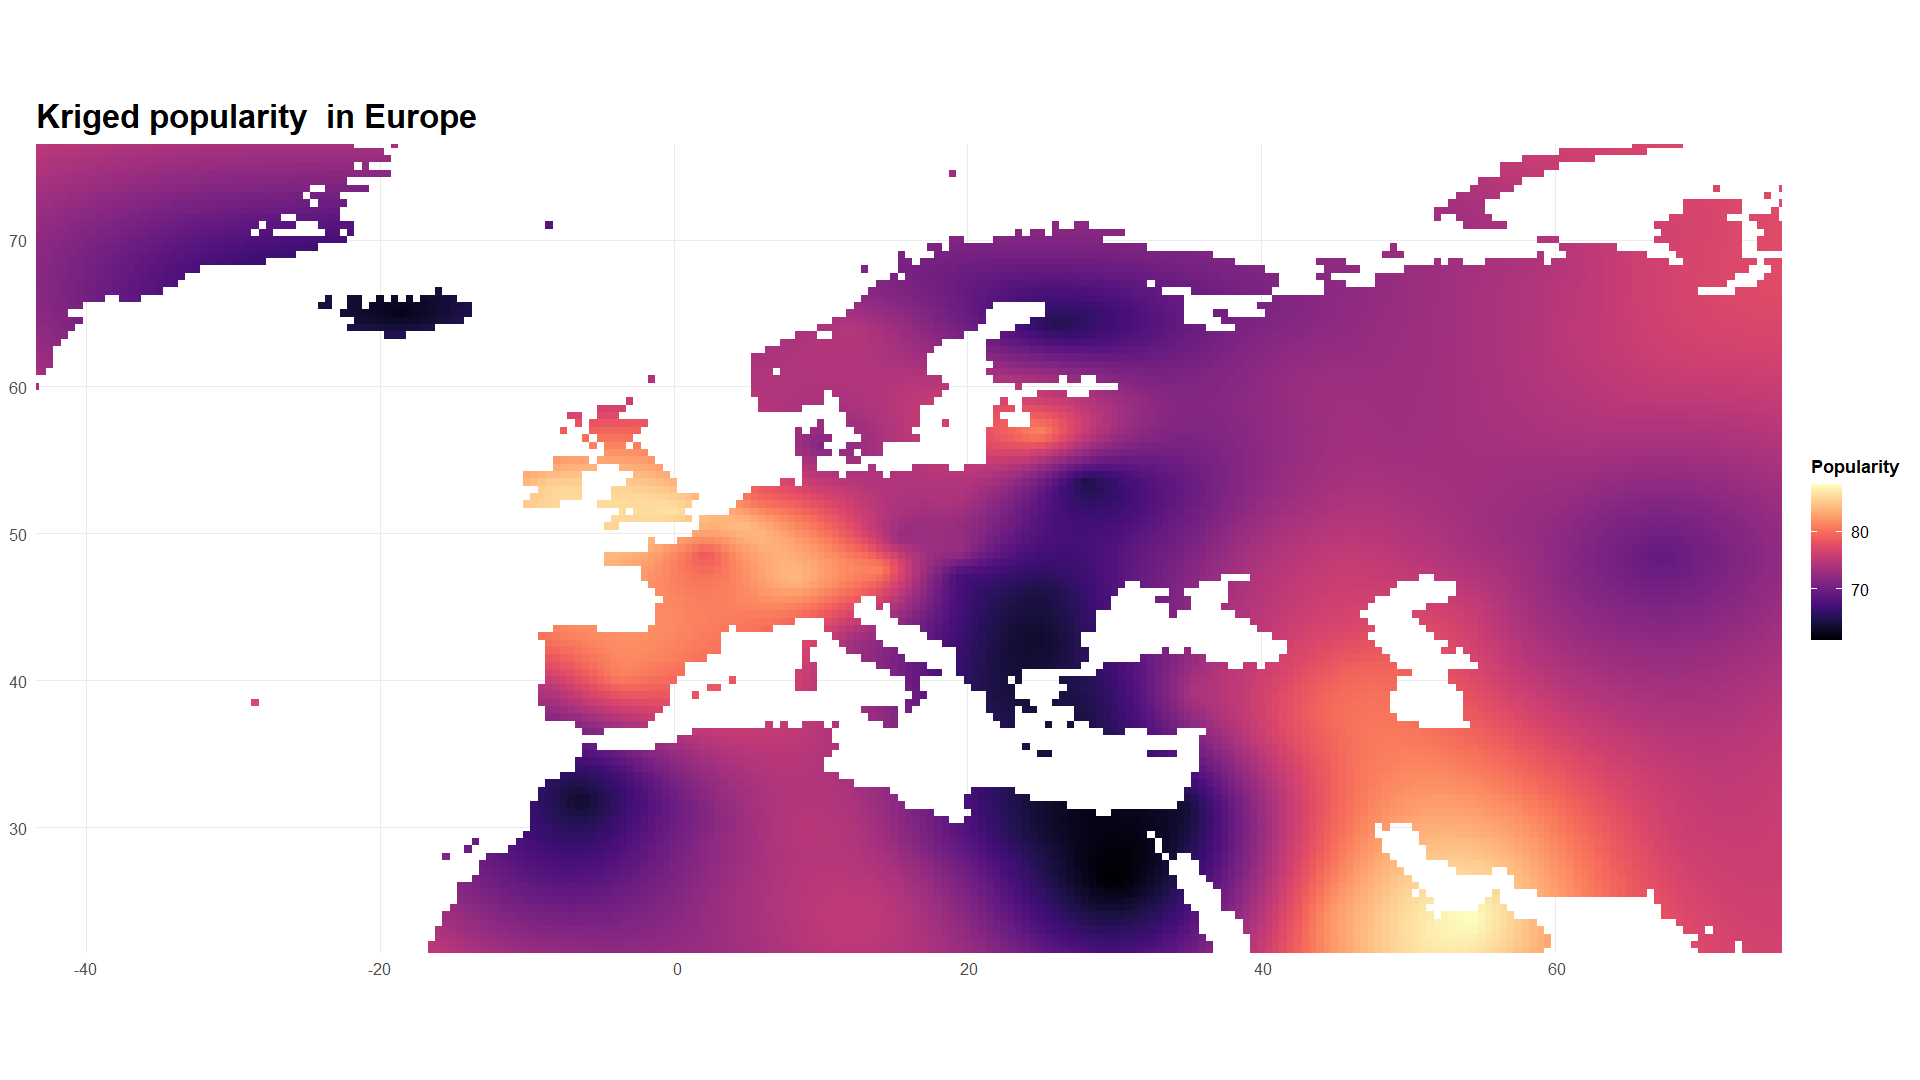
\includegraphics[width=0.75\linewidth]{Images//7_Geospatial//3_new/popularity_interpolation_europe.png}
    \caption{Interpol·lació usant kriging de la popularitat (Europa)}
    \label{fig:geo_new_pop_interpol_eur}
\end{figure}

Centrant-nos només en Europa \ref{fig:geo_new_pop_interpol_eur}, s'observa el que s'ha comentat abans: la zona de l'est té popularitats més baixes. Tot i això, destaca com a excepció la zona de Estonia, Letònia i Latvia, on s'observa una popularitat relativament alta. A l'oest, el Regne Unit destaca amb una popularitat molt alta, així com els Bèlgica, Països Baixos, Alemanya, Suïssa... França sembla tenir valors més baixos, així com Espanya i Portugal. Itàlia encara té menys popularitat, així com els països Nòrdics.

Aquests valors ens podem indicar, que les cançons més populars del món solen estar en anglès, fet que provoca que els països on es parla aquesta llengua tinguin popularitats més altes. A més, també tenen popularitats molt altes els països amb bastant immigració o turisme d'aquests, com podria ser Dubai.


\subsubsection{Valence}

Finalment, es va decidir ajustar un tercer model, aquest cop filtrant tan sols les dades d'Europa, per observar si es podia trobar certa relació utilitzant la positivitat de la música escoltada (valence).

El variograma, al tractar amb punts més propers entre ells, va ser realtizat amb un cutoff de 2000, i 250 de width. Analitzant-lo, es va escollir un model d'ona (Wave, Wav), ambuns valors de 0.0006 de psill, 700 de range i 0.0005 de nugget.

\begin{figure}[H]
    \centering
    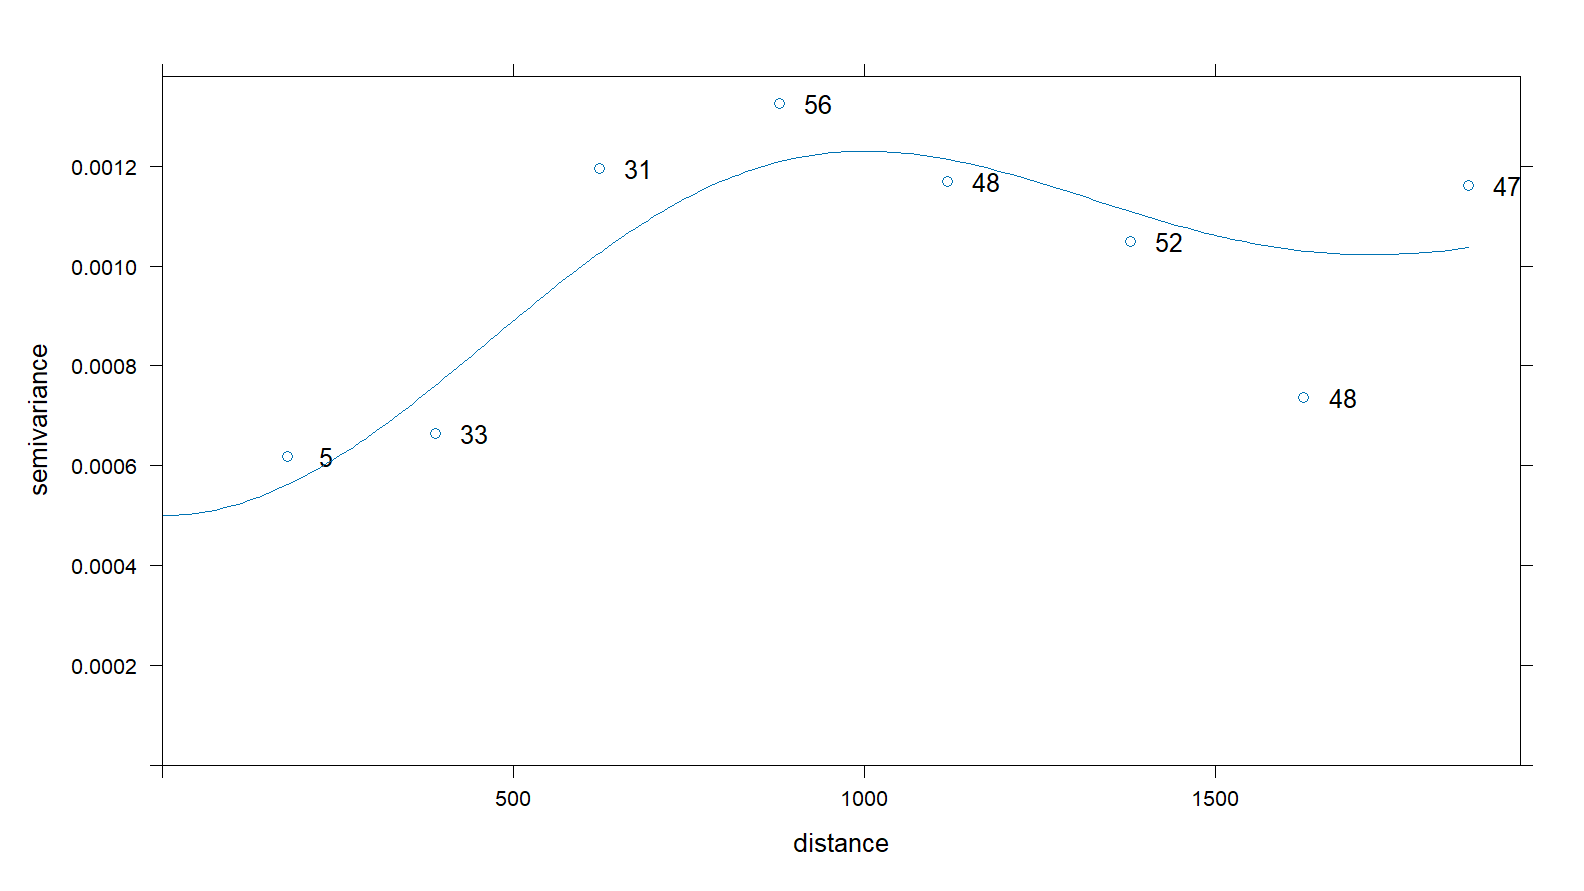
\includegraphics[width=0.5\linewidth]{Images//7_Geospatial//3_new/valence_variogram.png}
    \caption{Variograma ajustat per valence a Europa}
    \label{fig:geo_new_val_fit}
\end{figure}

Tot i que no s'ajusta perfectament, l'error mitjà és 0.0009, l'RMSE 0.03 i el MSRE 1.15, és a dir que té bastants bones mètriques. Per tant, s'ha escollit directament aquest per relitzar la interpol·lació \ref{fig:geo_new_valence_interpol}.

\begin{figure}[H]
    \centering
    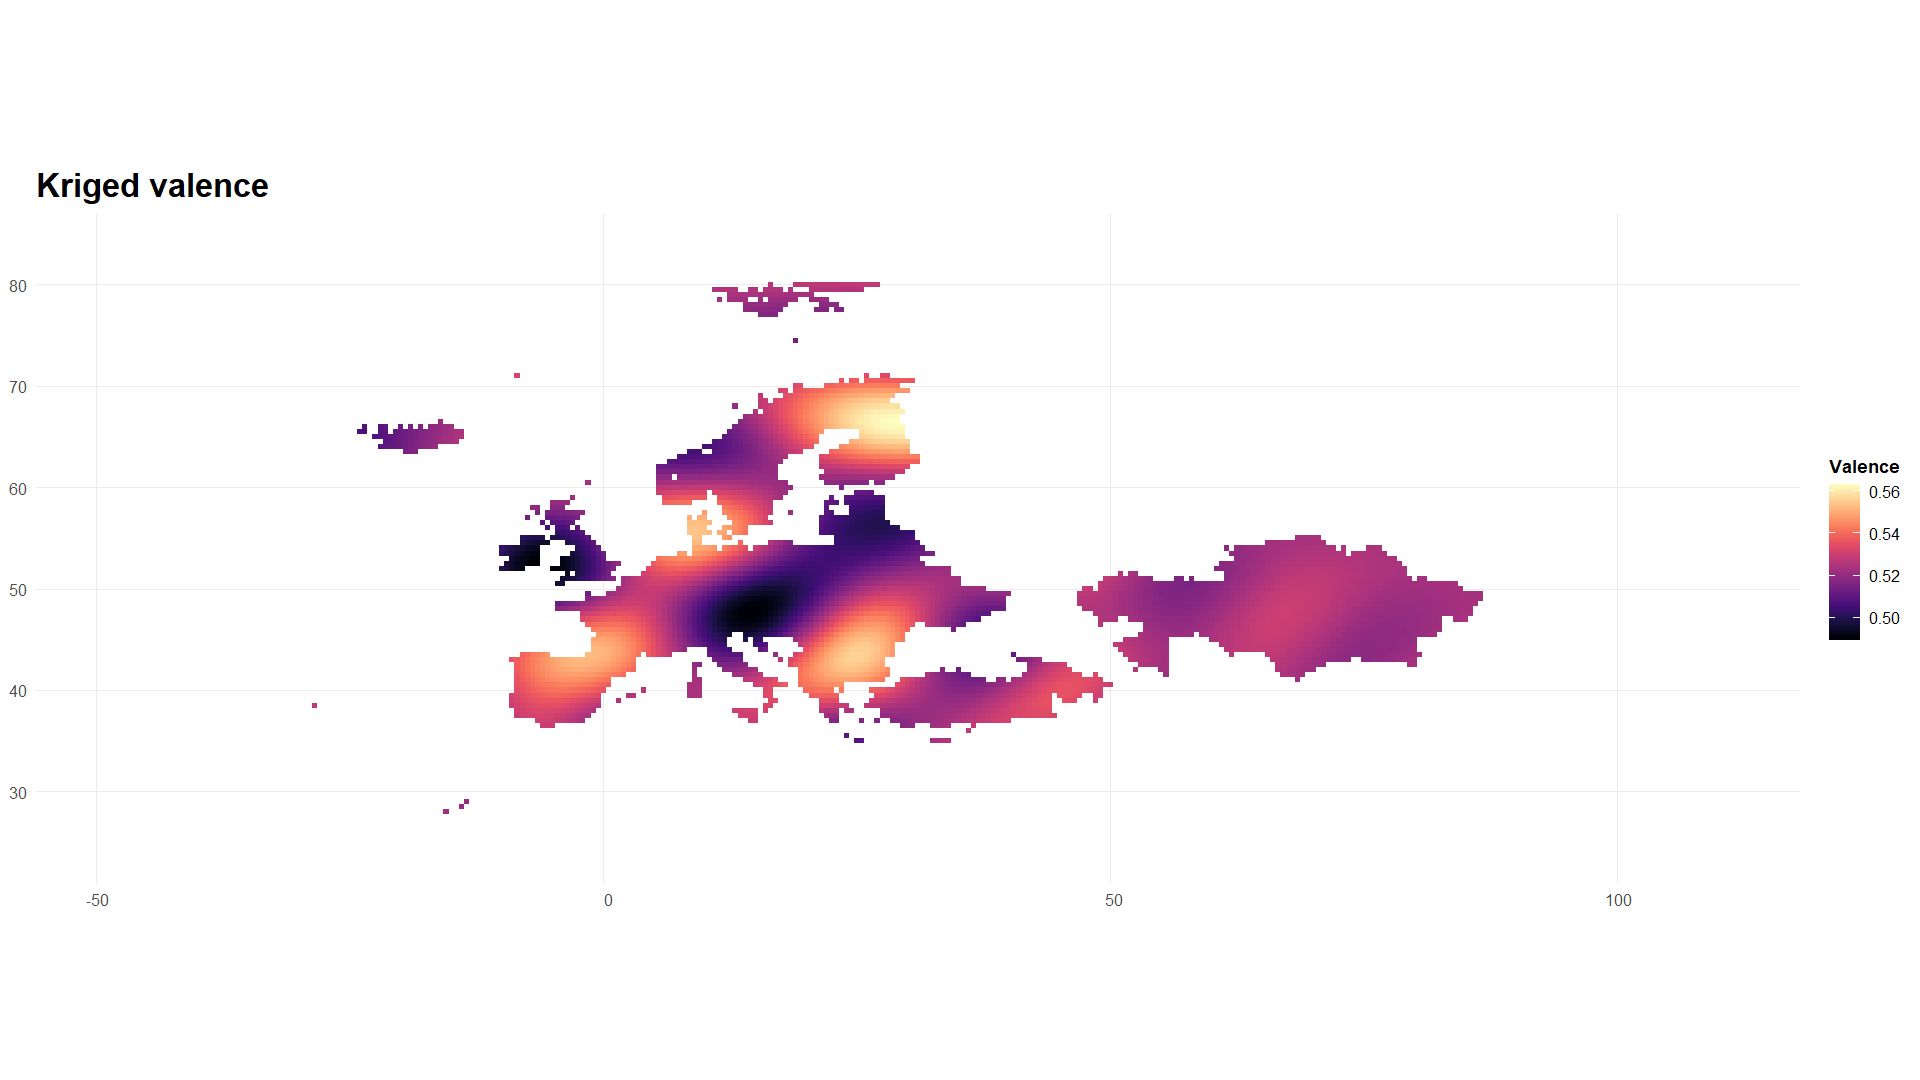
\includegraphics[width=0.8\linewidth]{Images//7_Geospatial//3_new/valence_interpolation.png}
    \caption{Interpol·lació usant kriging de valence a Europa}
    \label{fig:geo_new_valence_interpol}
\end{figure}

En aquesta observem 4 concentracions de positivitat: la península ibèrica, els balcans, Dinamarca i Finlàndia. Al l'inversa passa amb les zones del centre d'Europa (Àustria, Polònia, Hongria...) i amb el Regne Unit. 

Per interpretar aquests valors, cal conèixer diverses dades. D'entrada, sembla ser que Dinamarca i Finlàndia escolten cançons més positives perquè solen ser països amb gent feliç. De fet, segons , són actualment el segon i primer país més feliç del món. Per tant, no és d'extranyar que la gent feliç escolti música positiva, ja que solem escoltar música en funció de l'estat d'ànim en el que ens trobem \cite{worldhappiness2024}.

Tot i això, aquesta explicació no ens serveix pels balcans (segons el mateix estudi, la gent no és gaire feliç en aquella zona), ni per Islàndia, un altre país aparentment feliç. Per entendre aquests casos, així com la península ibèrica, cal entendre que són llocs amb cultures diferents: els feliços solen ser llocs amb una forta identitat cultural i festiva, més mediterrània, oberta i amb música local ballable; d'altra banda, els tristos solen ser zones més fredes i amb climes més durs, o més clàssiques.


